% TP_Oscillateurs_Manipulation_KALIPE.tex
\documentclass[11pt,a4paper]{report}

% -------- Packages --------
\usepackage[utf8]{inputenc}
\usepackage[T1]{fontenc}
\usepackage[french]{babel}
\usepackage{geometry}
\usepackage{graphicx}
\usepackage{amsmath,amssymb}
\usepackage{siunitx}
\usepackage{float}
\usepackage{fancyhdr}
\usepackage{booktabs}
\usepackage{array}
\usepackage{caption}
\usepackage{subcaption}
\usepackage{tcolorbox}
\usepackage{hyperref}
\usepackage{longtable}
\usepackage{multirow}

\geometry{margin=2cm}
\hypersetup{colorlinks=true, linkcolor=black, urlcolor=blue}

% -------- En-têtes --------
\pagestyle{fancy}
\fancyhf{}
\fancyhead[L]{TP — Oscillateurs Sinusoïdaux}
\fancyfoot[C]{\thepage}

% -------- Commandes utiles --------
\newcommand{\HRule}{\rule{\linewidth}{0.5mm}}
\newtcolorbox{objectifbox}{colback=gray!5,colframe=black!60,title=Objectifs pédagogiques}

% -------- Document --------
\begin{document}

% ---------- Page de garde ----------
\begin{titlepage}
    \centering
    \vspace*{1cm}
    
    
    {\Large \textsc{Sorbonne Université}}\\[0.5cm]
    {\large Master 1 SYSCOM}\\[0.3cm]
    {\large Électronique des Systèmes Analogiques}\\[2cm]
    
    \HRule \\[0.6cm]
    {\Huge \textbf{Travaux Pratiques}}\\[0.4cm]
    {\huge \textbf{Oscillateurs Sinusoïdaux}}\\[0.4cm]
    \HRule \\[1.5cm]
    
    {\Large \textbf{Partie Manipulation}}\\[2.5cm]
    
    \begin{tabular}{ll}
        \multicolumn{2}{c}{\textbf{\large Réalisé par :}} \\[0.5cm]
        \textbf{Étudiant :} & Kossi Mathias KALIPE \\
        \textbf{N° :} & 21507247 \\[0.5cm]
        \textbf{Étudiant :} & Abdelrahman ABDELMAGID \\
        \textbf{N° :} & 21204758 \\
    \end{tabular}
    
    \vfill
    
    {\large Année universitaire 2025--2026}\\[0.3cm]
    
\end{titlepage}

% ---------- Résumé ----------
\begin{abstract}
Ce document présente la partie expérimentale du TP sur les oscillateurs sinusoïdaux :
oscillateur à pont de Wien (avec stabilisation d'amplitude par FET) et oscillateur
à déphasage RC. Les mesures réalisées en laboratoire (fréquences, amplitudes, gains
et comportement lors de variations de paramètres) sont consignées et comparées aux
prédictions théoriques. Des captures d'oscilloscope sont prévues pour
illustrer les formes d'onde et le démarrage des oscillations.
\end{abstract}

\tableofcontents
\thispagestyle{empty}
\clearpage

% ---------- Introduction ----------
\chapter*{Introduction}
\addcontentsline{toc}{chapter}{Introduction}

Les oscillateurs sinusoïdaux sont des éléments fondamentaux en électronique analogique.
Ils permettent de générer des signaux périodiques sans entrée sinusoïdale. Ce TP a
pour objectif d'étudier expérimentalement deux architectures classiques : le pont de
Wien et l'oscillateur à déphasage. Nous vérifions les conditions de Barkhausen,
mettons en place une régulation d'amplitude automatique et analysons l'influence des
caractéristiques des amplificateurs opérationnels (GBW, Slew Rate) sur la qualité
du signal de sortie.

\begin{objectifbox}
\begin{itemize}
    \item Vérifier expérimentalement la fréquence d'oscillation des réseaux RC (Wien et déphasage).
    \item Mettre en évidence la condition d'amplitude ($|A\beta|=1$) et la condition de phase.
    \item Implémenter une stabilisation d'amplitude par résistance commandée en tension (FET).
    \item Étudier l'influence du produit gain-bande et du Slew Rate (TL081 vs $\mu$A741).
    \item Mesurer et commenter le démarrage des oscillations et les distorsions observées.
\end{itemize}
\end{objectifbox}

\clearpage

% ---------- Matériel ----------
\chapter{Matériel et montage}
\section*{Matériel utilisé}
\begin{itemize}
    \item Générateur BF (0--20 kHz)
    \item Oscilloscope 2 voies (mode XY et mode temporel)
    \item TL081 (AOP) et $\mu$A741 (remplaçant)
    \item Résistances : plusieurs (220 \(\Omega\), 1 k\(\Omega\), 2.2 k\(\Omega\), 3.9 k\(\Omega\), etc.)
    \item Potentiomètres : 1 k\(\Omega\), 10 k\(\Omega\)
    \item Capacités : \(\SI{4.7}{\nano\farad}\), \(\SI{1}{\nano\farad}\), \(\SI{10}{\nano\farad}\), \(\SI{330}{\nano\farad}\), \(\SI{4.7}{\micro\farad}\)
    \item JFET (ex. 2N5457 ou 2N3819 selon disponibilité) pour R commandée en tension
    \item Alimentation symétrique ±12 V
    \item Breadboard, câbles, multimètre
\end{itemize}

\section*{Notation expérimentale}
Dans les tables, les fréquences sont en hertz (Hz), les tensions en volts (V), et les résistances en ohms (\\Omega\\). Les mesures sont réalisées à température ambiante, sans correction d'incertitude systématique détaillée (valeurs arrondies à 2–3 chiffres significatifs).

\clearpage

% ---------- Partie A : Wien ----------
\chapter{Oscillateur à pont de Wien}

\section{Montage et conditions initiales}
Le réseau de réaction (pont de Wien) utilisé en labo est celui étudié en cours :
deux branches \(R\!-\!C\) (une série, une parallèle) connectées entre la sortie et l'entrée non
inverseuse de l'amplificateur. Pour les essais initiaux on a pris :
\[
R = \SI{3.9}{\kilo\ohm}, \qquad C = \SI{4.7}{\nano\farad}
\]
Ces valeurs correspondent au sujet fourni et donnent une fréquence théorique :
\[
f_{th} = \frac{1}{2\pi RC} \approx \frac{1}{2\pi \times 3900 \times 4.7\times 10^{-9}} \approx \SI{8.69}{\kilo\hertz}
\]

\subsection{I -- Mesure du réseau de réaction (mode XY)}

\begin{figure}[H]
    \centering
    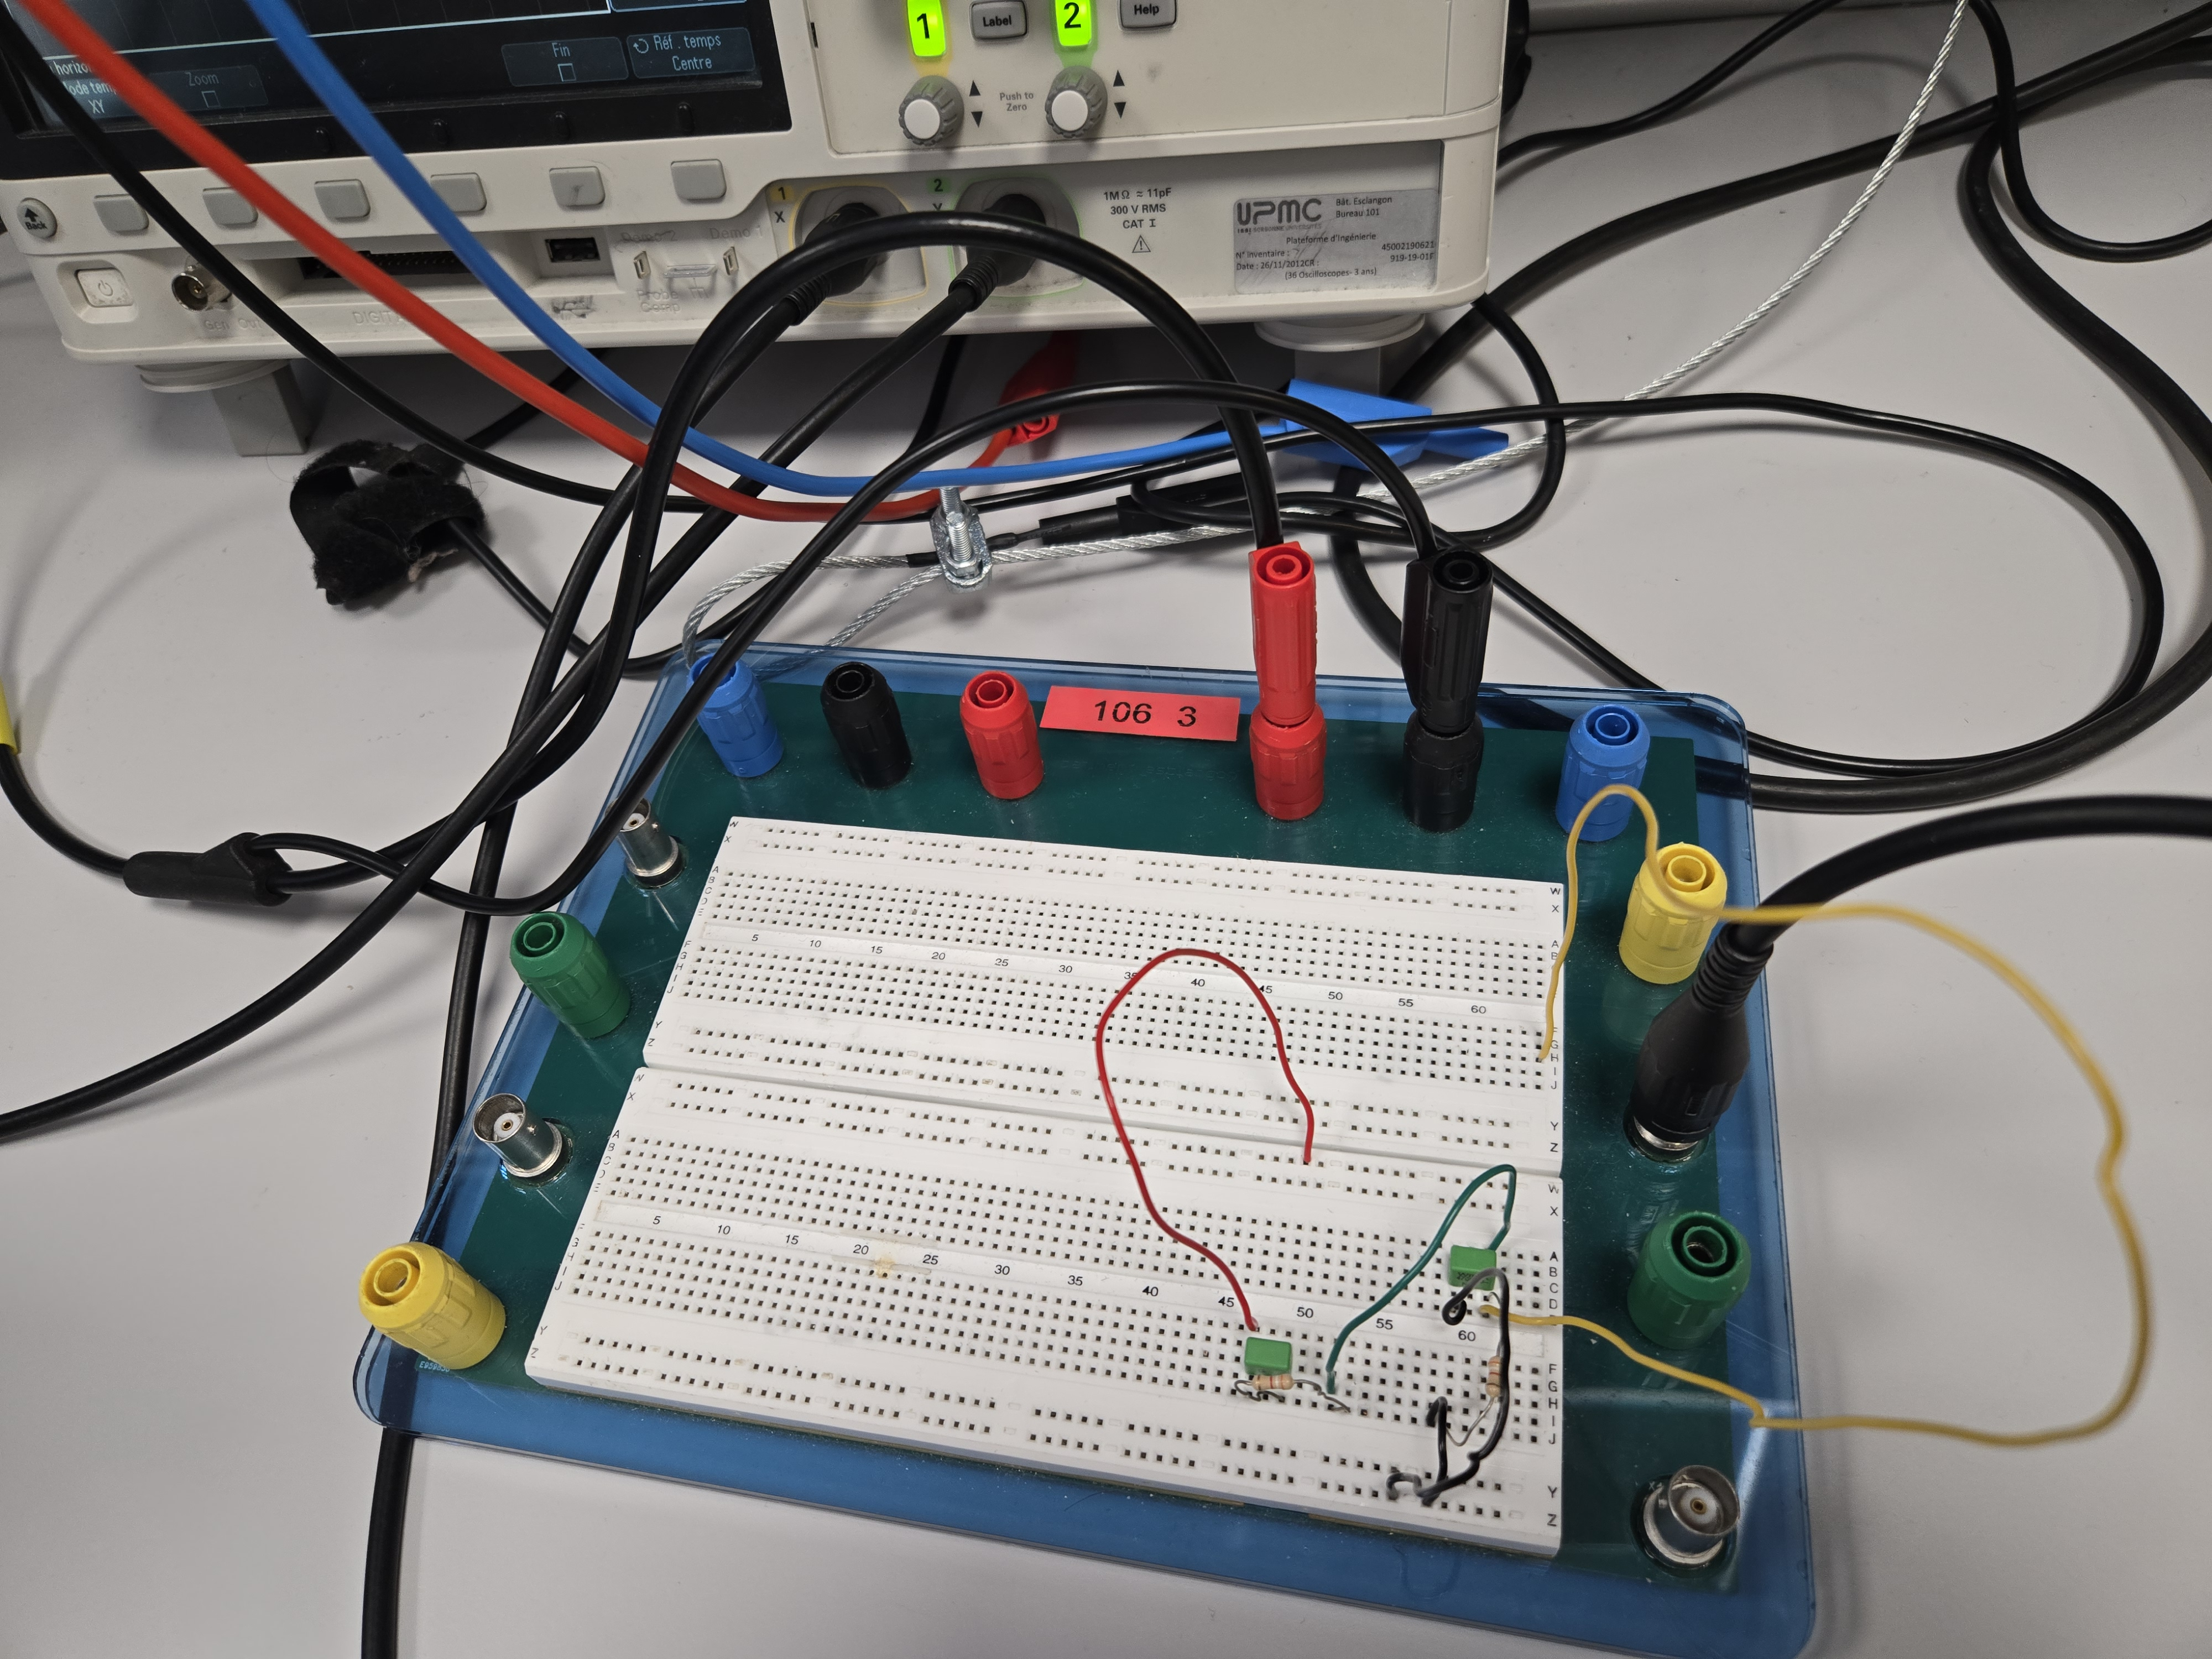
\includegraphics[width=0.78\linewidth]{images/reseau_reaction_rc.jpg}
    \caption{Circuit du réseau de réaction.}
\end{figure}

Procédure :
\begin{enumerate}
    \item On alimente le réseau par un GBF, on place l'oscilloscope en mode XY : $V_{in}$ sur X, $V_{out}$ sur Y.
    \item On balaye la fréquence autour de la valeur théorique pour repérer la fréquence où la trace devient alignée (phase nulle relative).
    \item On lit la fréquence du GBF et le rapport d'amplitude $|\beta| = V_{out}/V_{in}$ à cette fréquence.
\end{enumerate}

\paragraph{Mesures (réseau seul)}
\begin{table}[H]
\centering
\begin{tabular}{lcc}
\toprule
Grandeur & Valeur mesurée & Commentaire \\
\midrule
Fréquence théorique $f_{th}$ & \SI{8.69}{\kilo\hertz} & calculée \\
Fréquence mesurée $f_{m}$ & \SI{8.90}{\kilo\hertz} & mode XY (alignement) \\
Rapport d'atténuation $|\beta|$ & 0.333 & proche de $1/3$ attendu \\
Phase & $0^\circ$ (à $f_m$) & vérifié par XY / Lissajous \\
\bottomrule
\end{tabular}
\caption{Mesures sur le réseau de réaction (Wien)}
\end{table}

\begin{figure}[H]
    \centering
    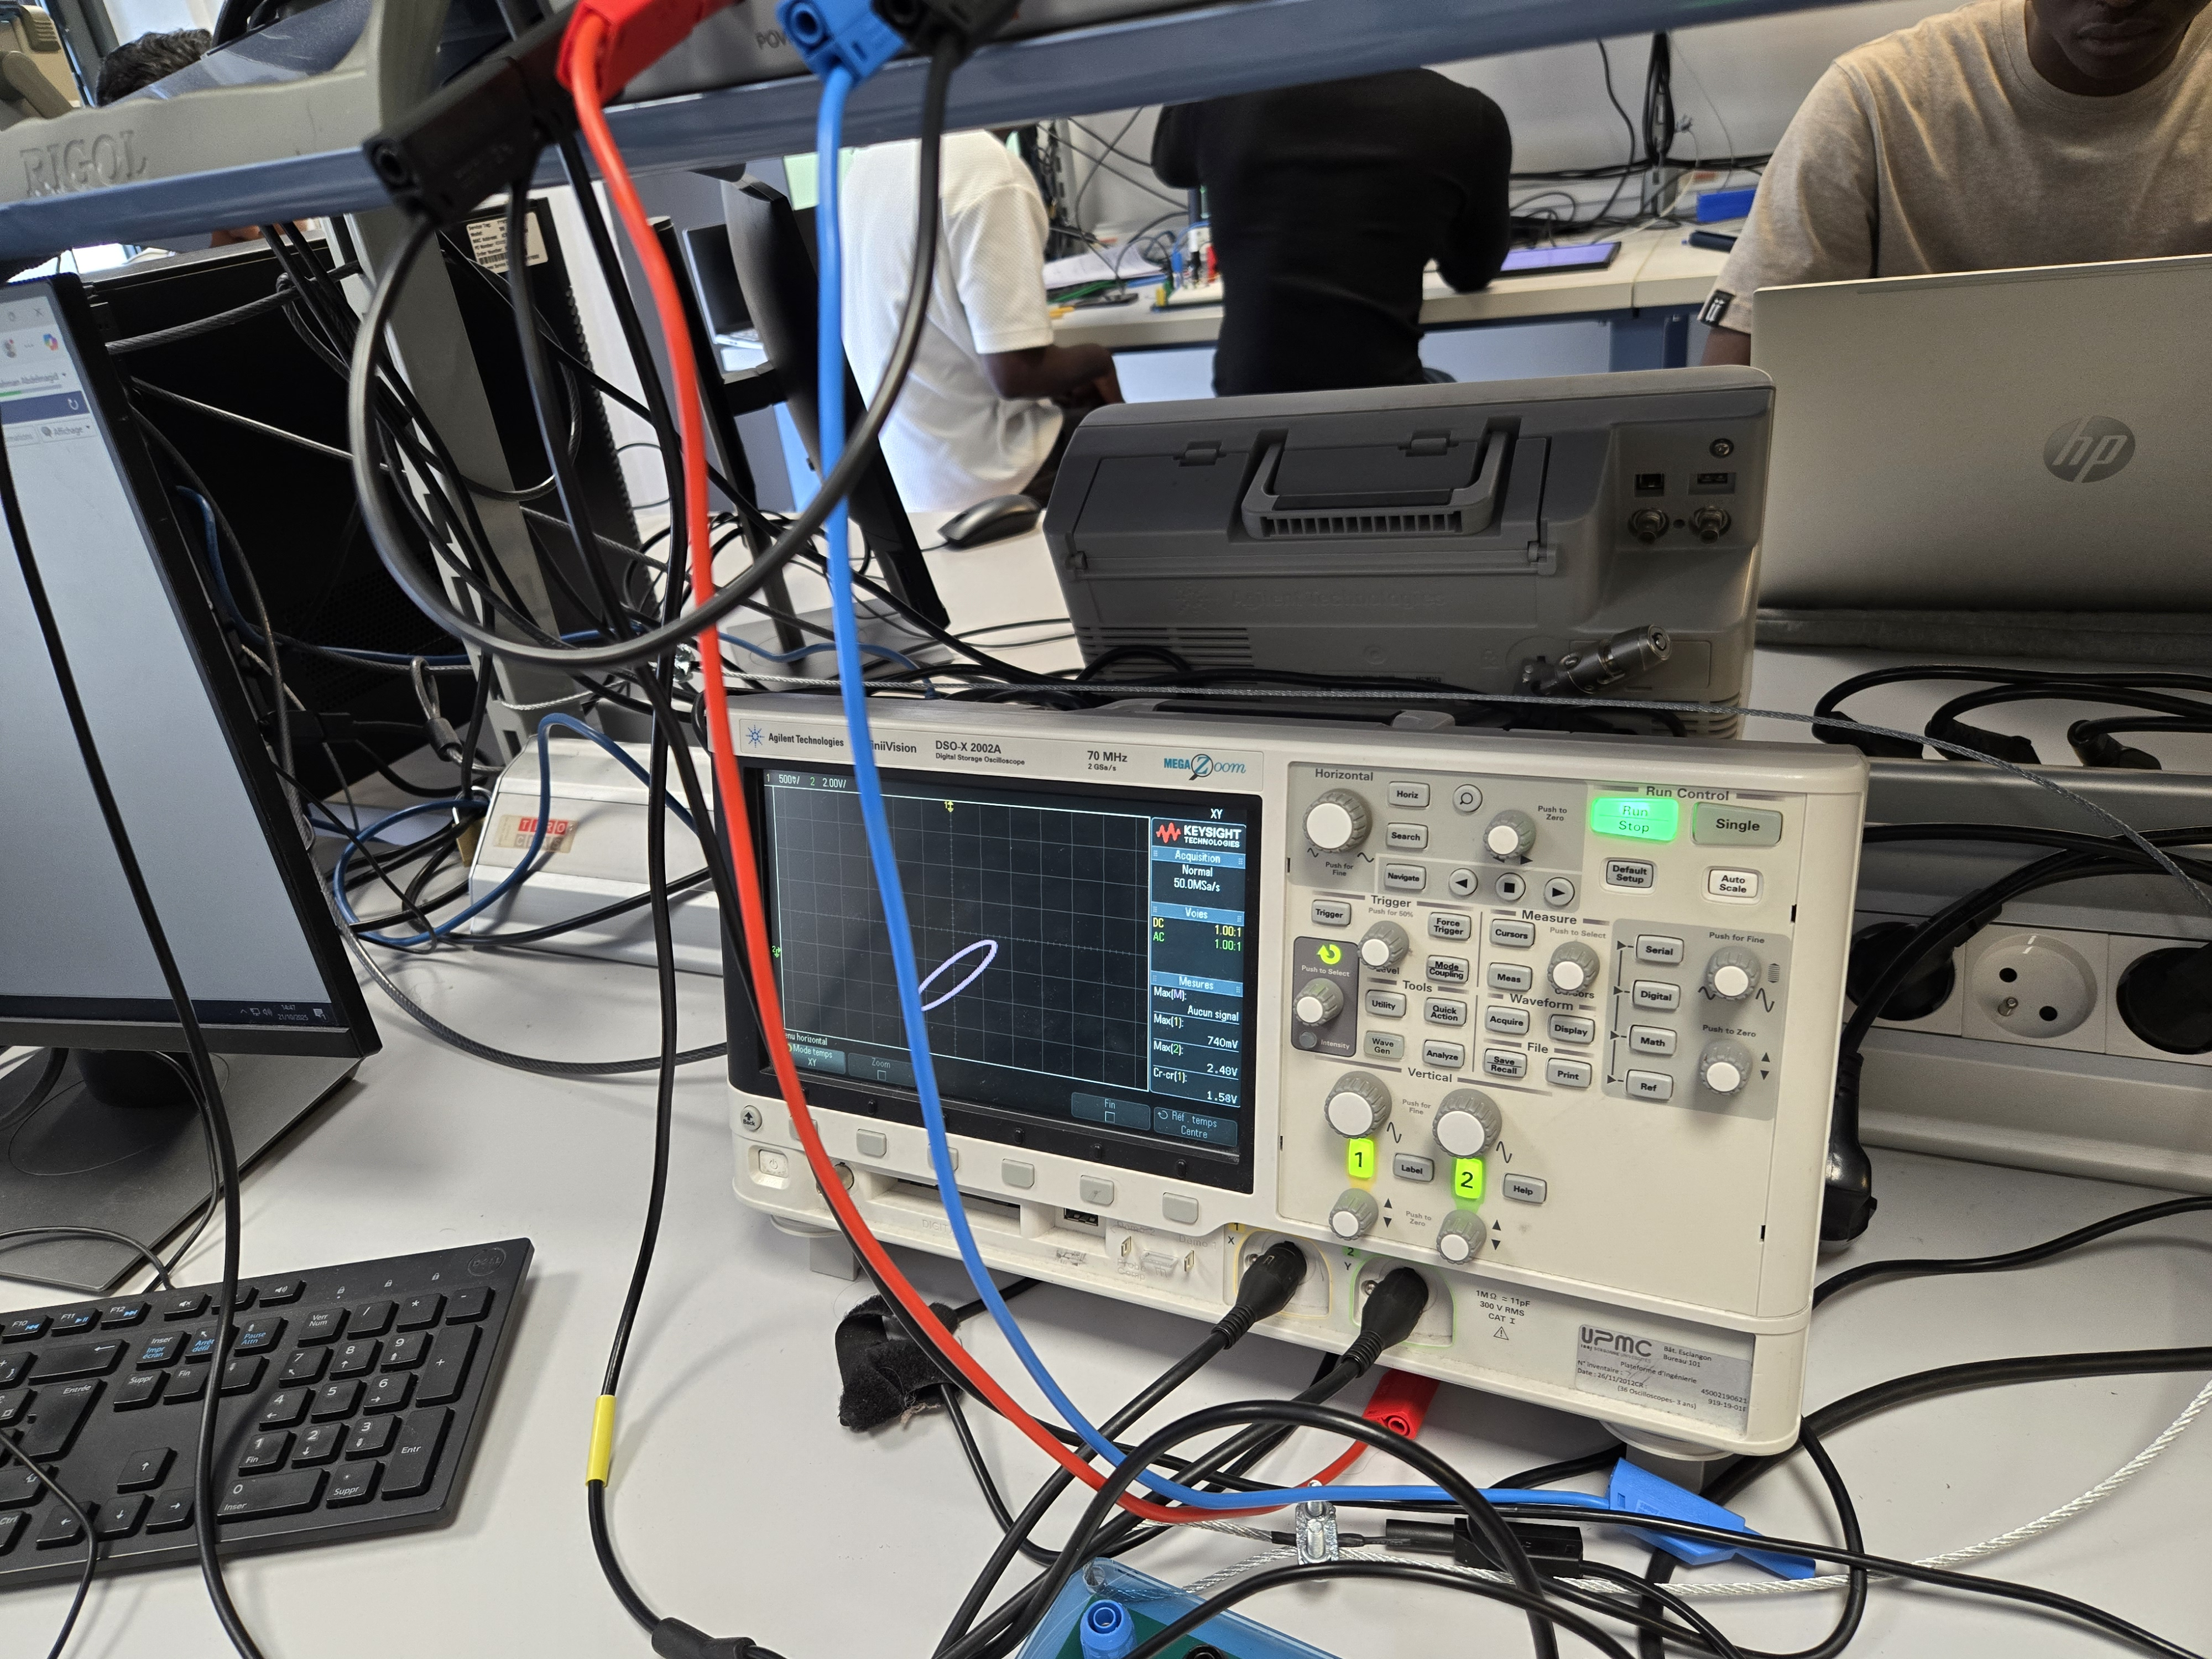
\includegraphics[width=0.78\linewidth]{images/reseau_reaction_xy_1.jpg}
    \caption{Tracé XY du réseau de réaction (Wien).}
\end{figure}

\begin{figure}[H]
    \centering
    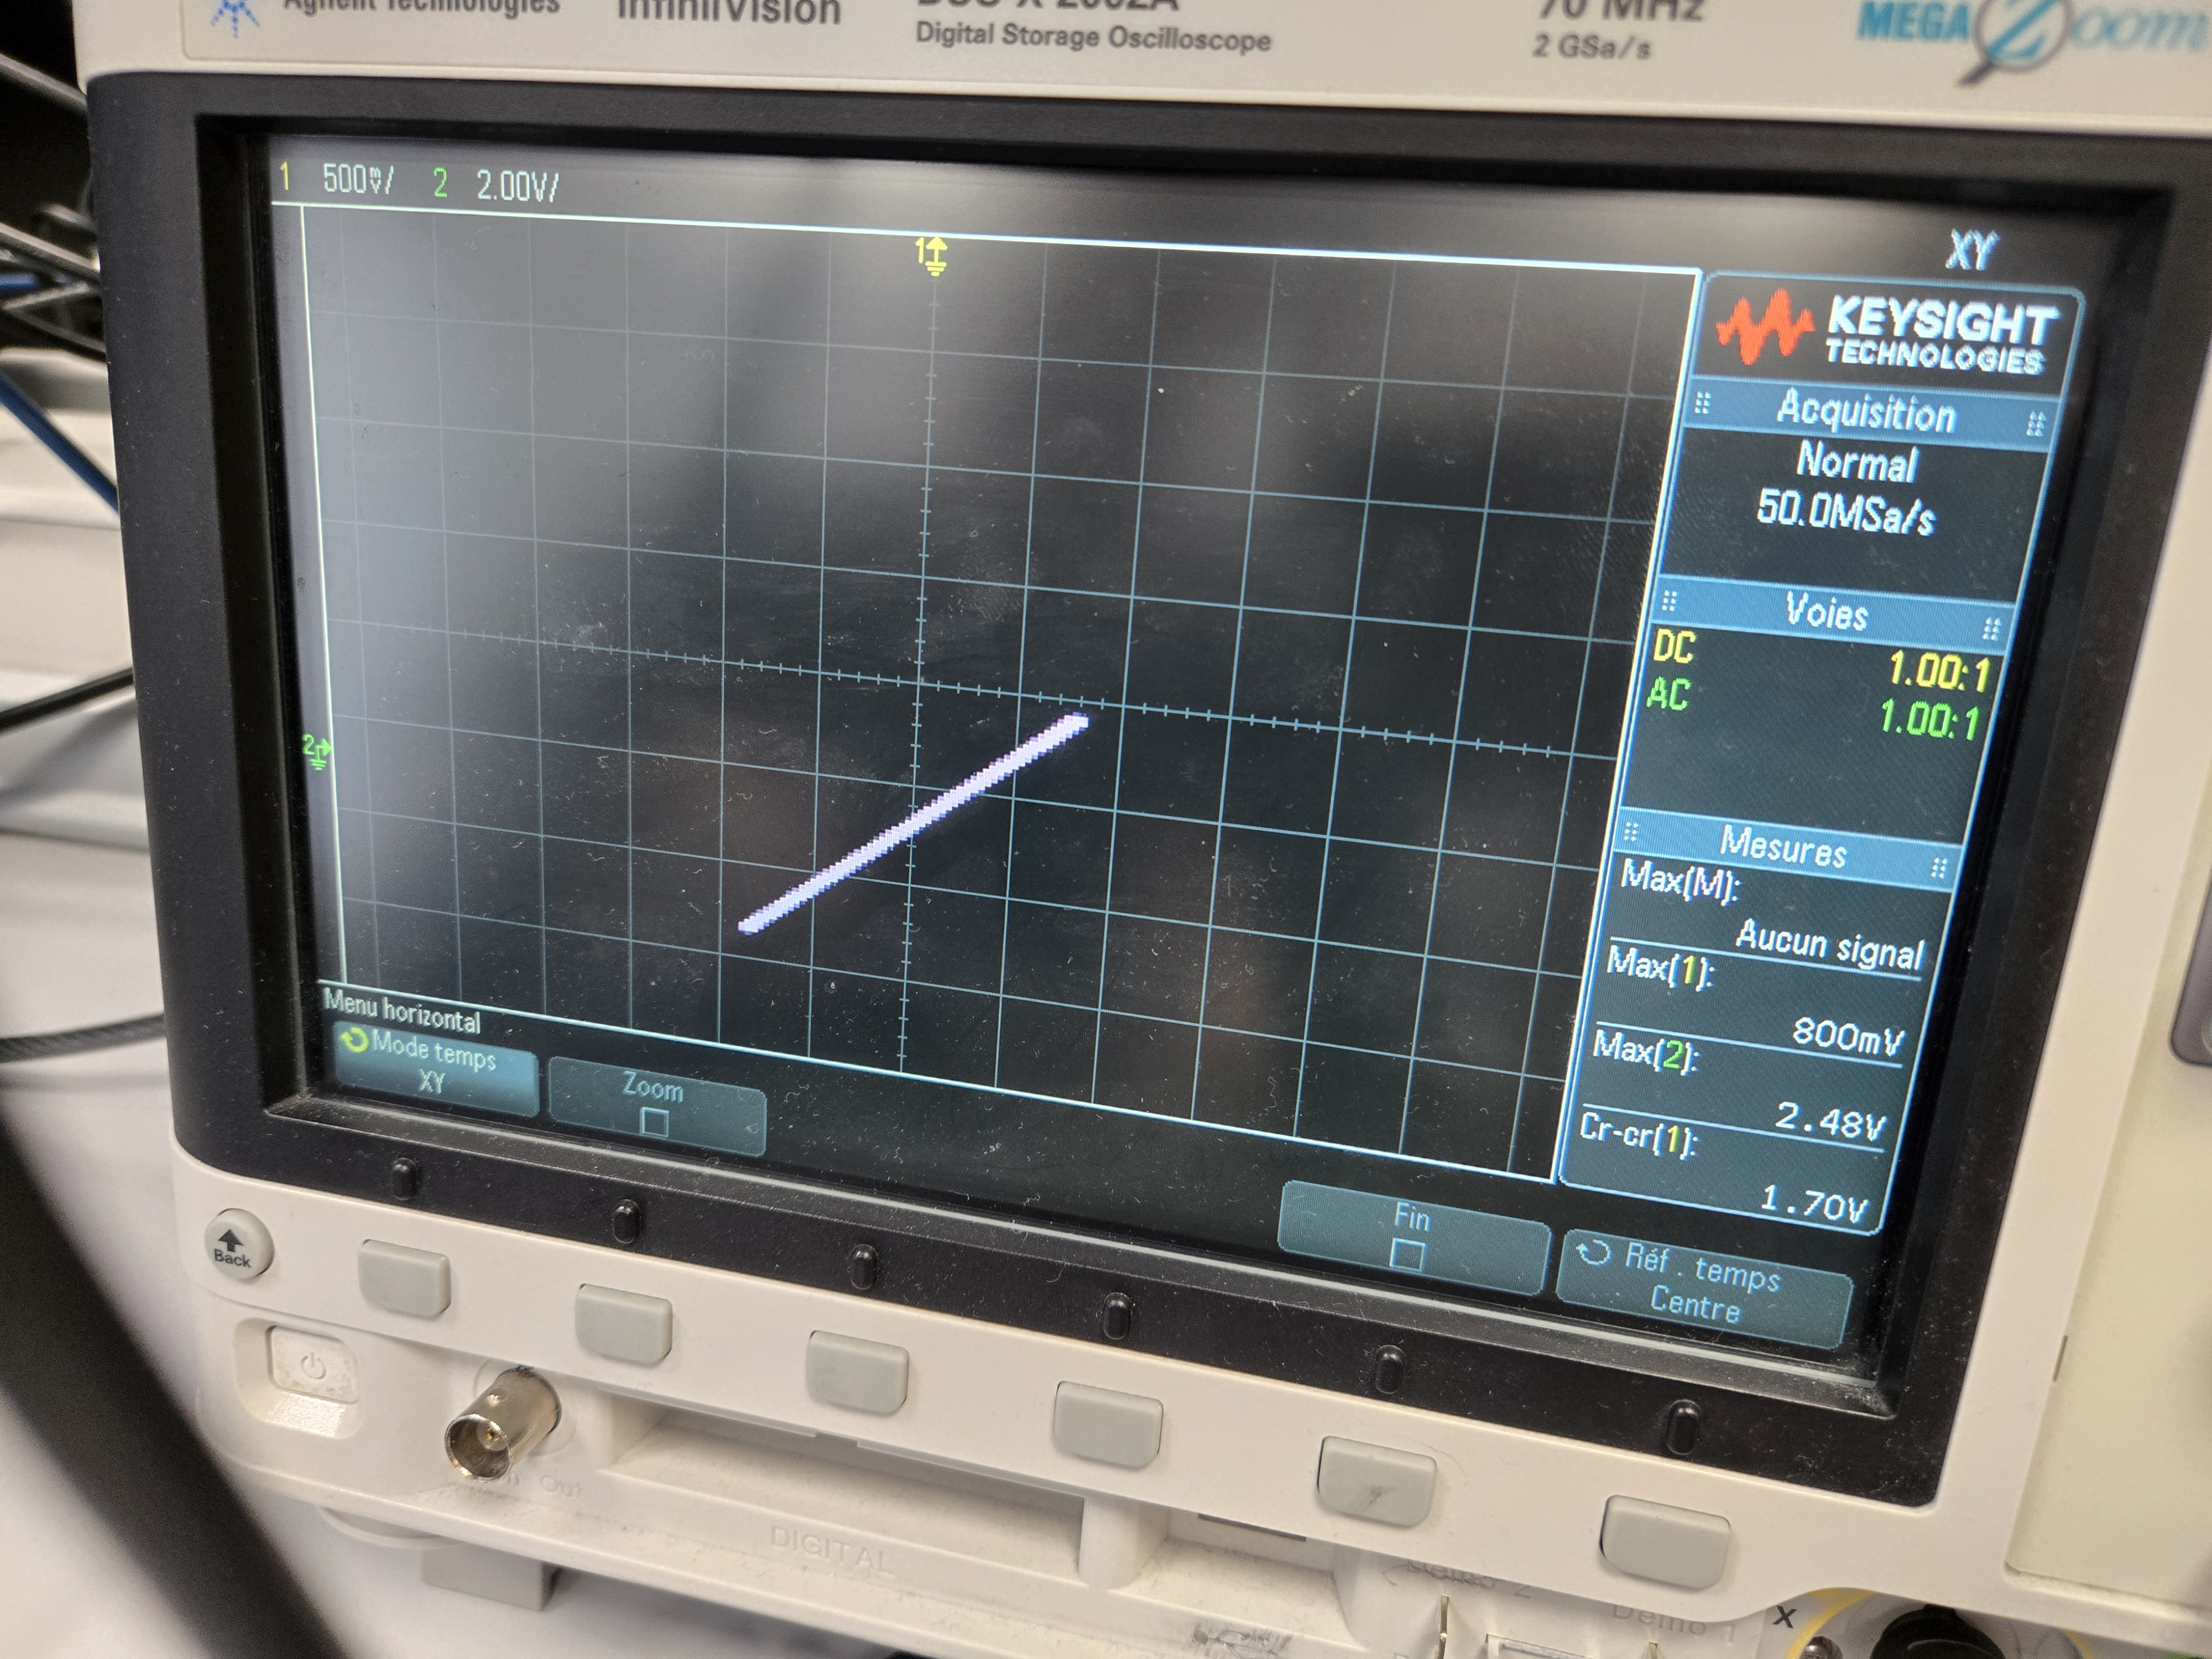
\includegraphics[width=0.78\linewidth]{images/reseau_reaction_xy2.jpg}
    \caption{Tracé XY du réseau de réaction (Wien) à $f\approx \SI{8.90}{\kilo\hertz}$.}
\end{figure}
\begin{figure}[H]
    \centering
    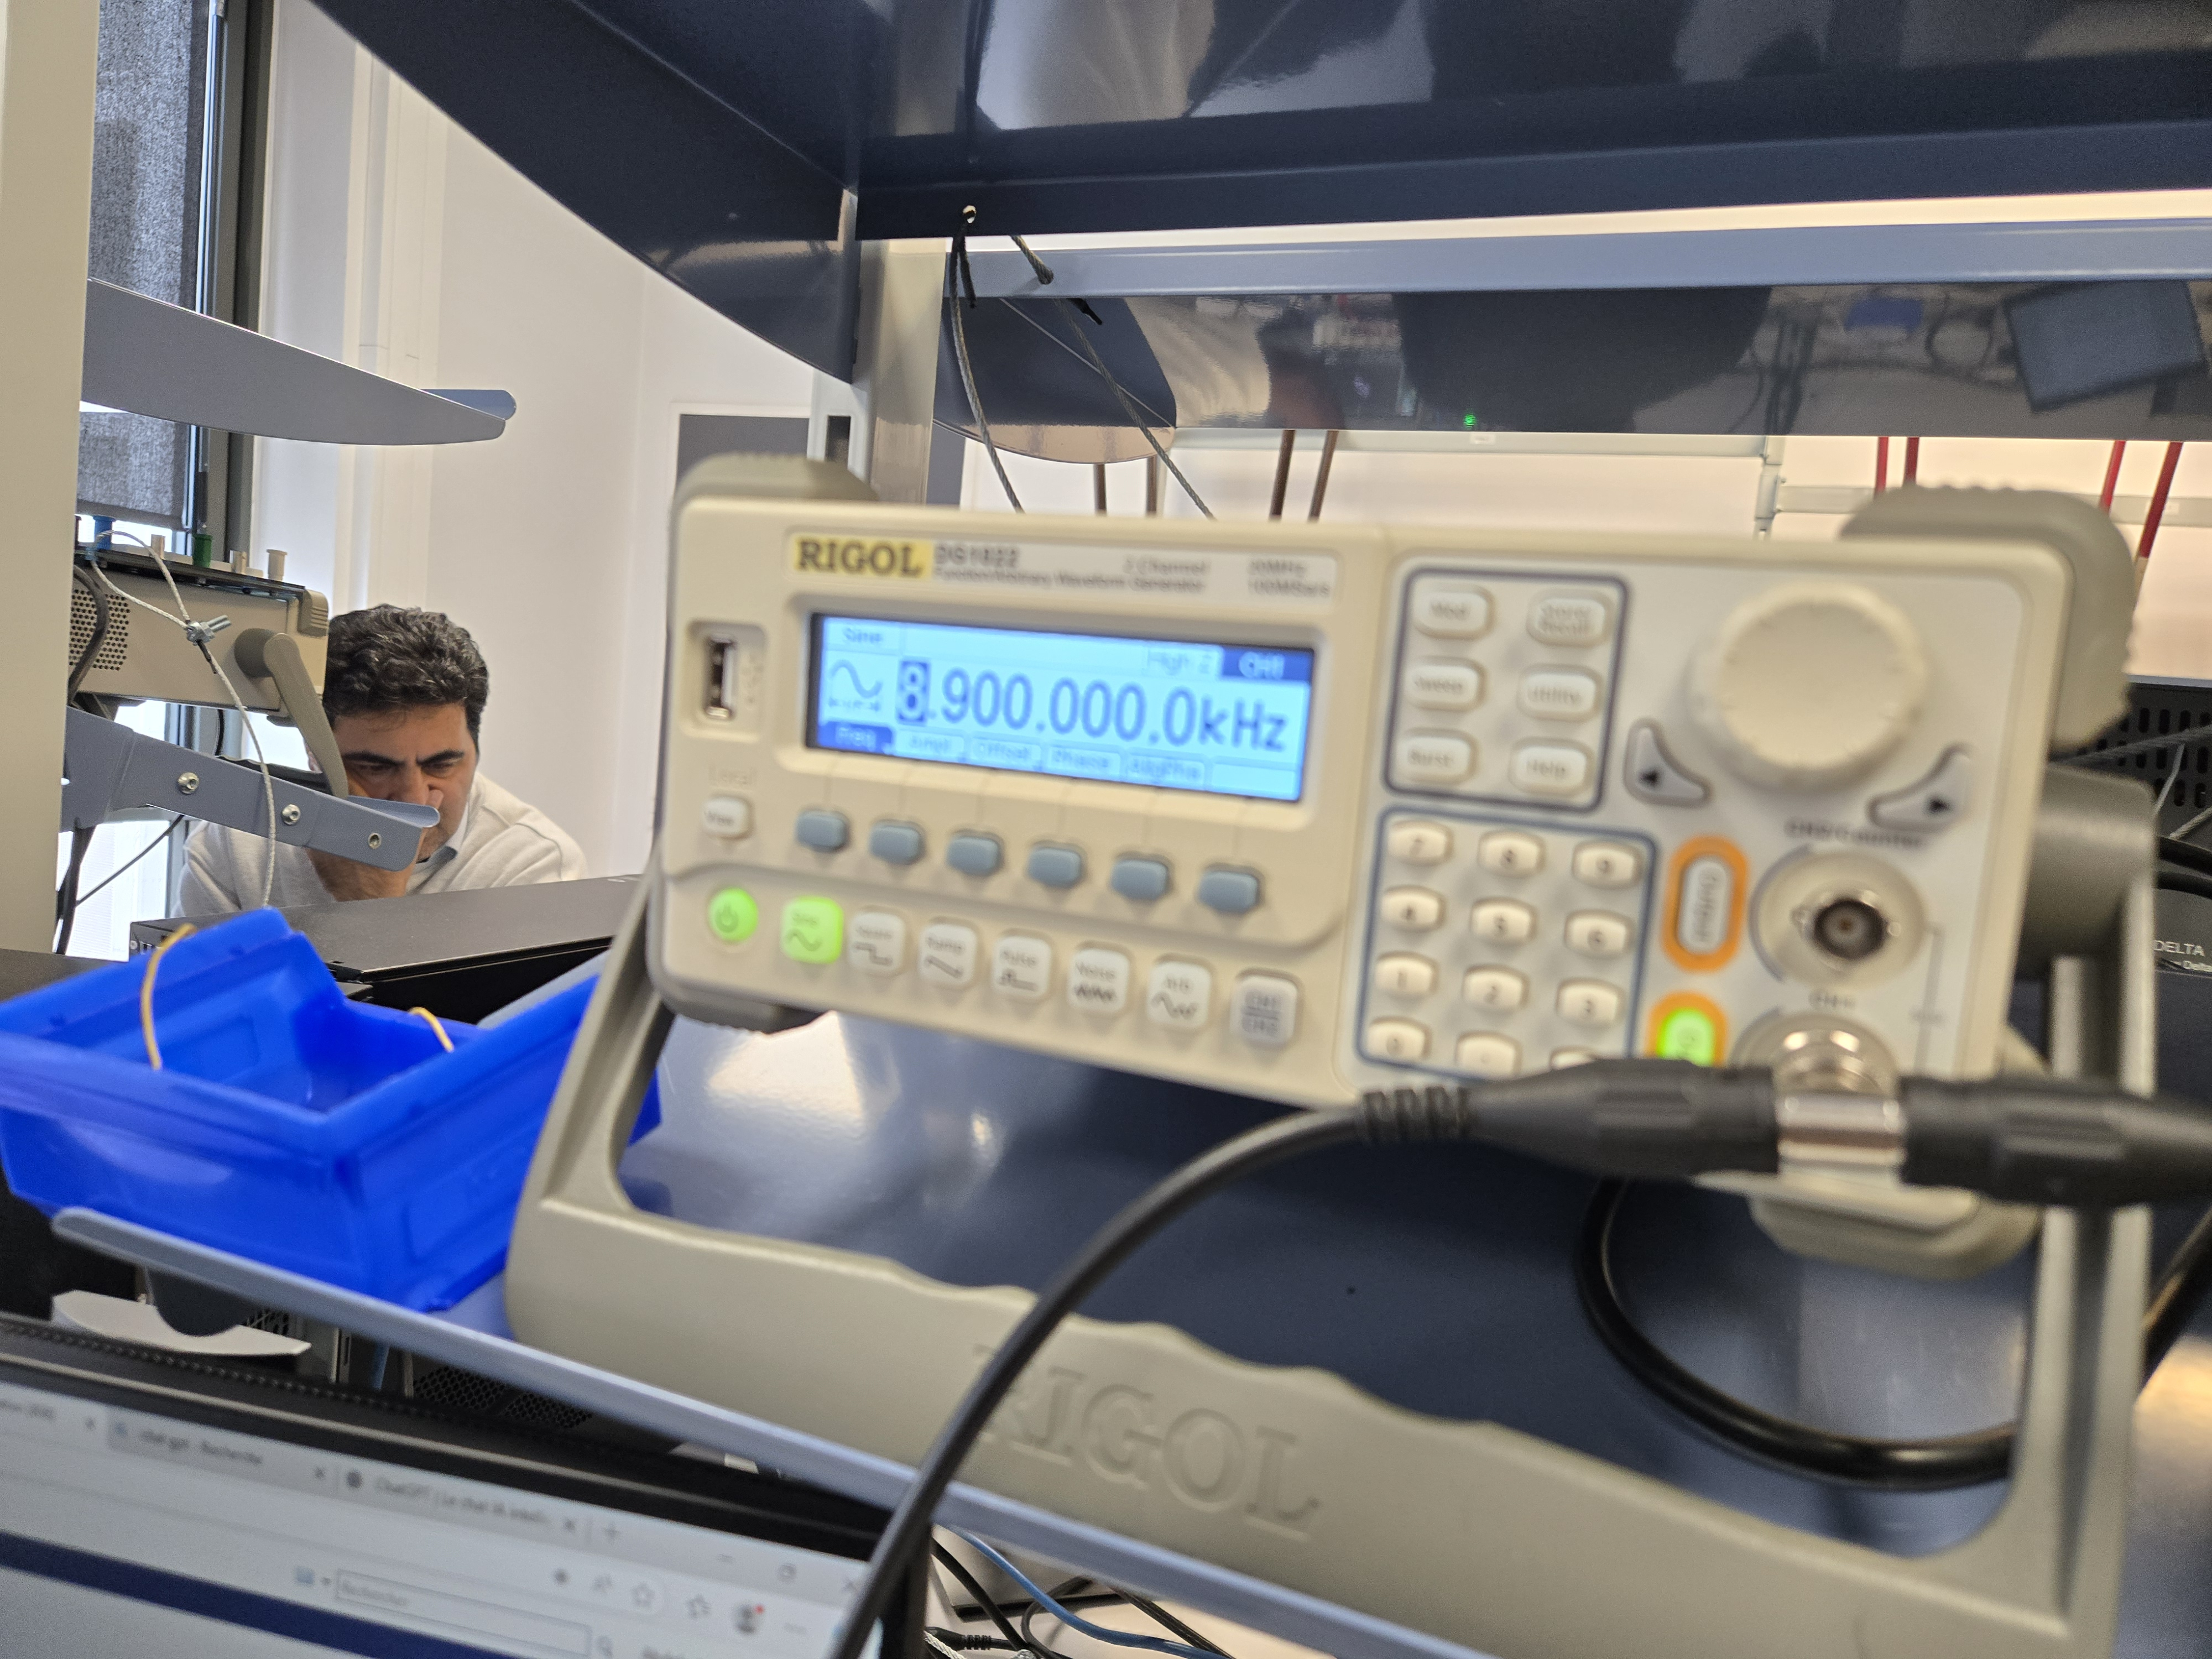
\includegraphics[width=0.78\linewidth]{images/reseau_reaction_fosc.jpg}
    \caption{Fréquence du réseau de réaction.}
\end{figure}

\subsection{II -- Montage complet et réglage du gain}

\begin{figure}[H]
    \centering
    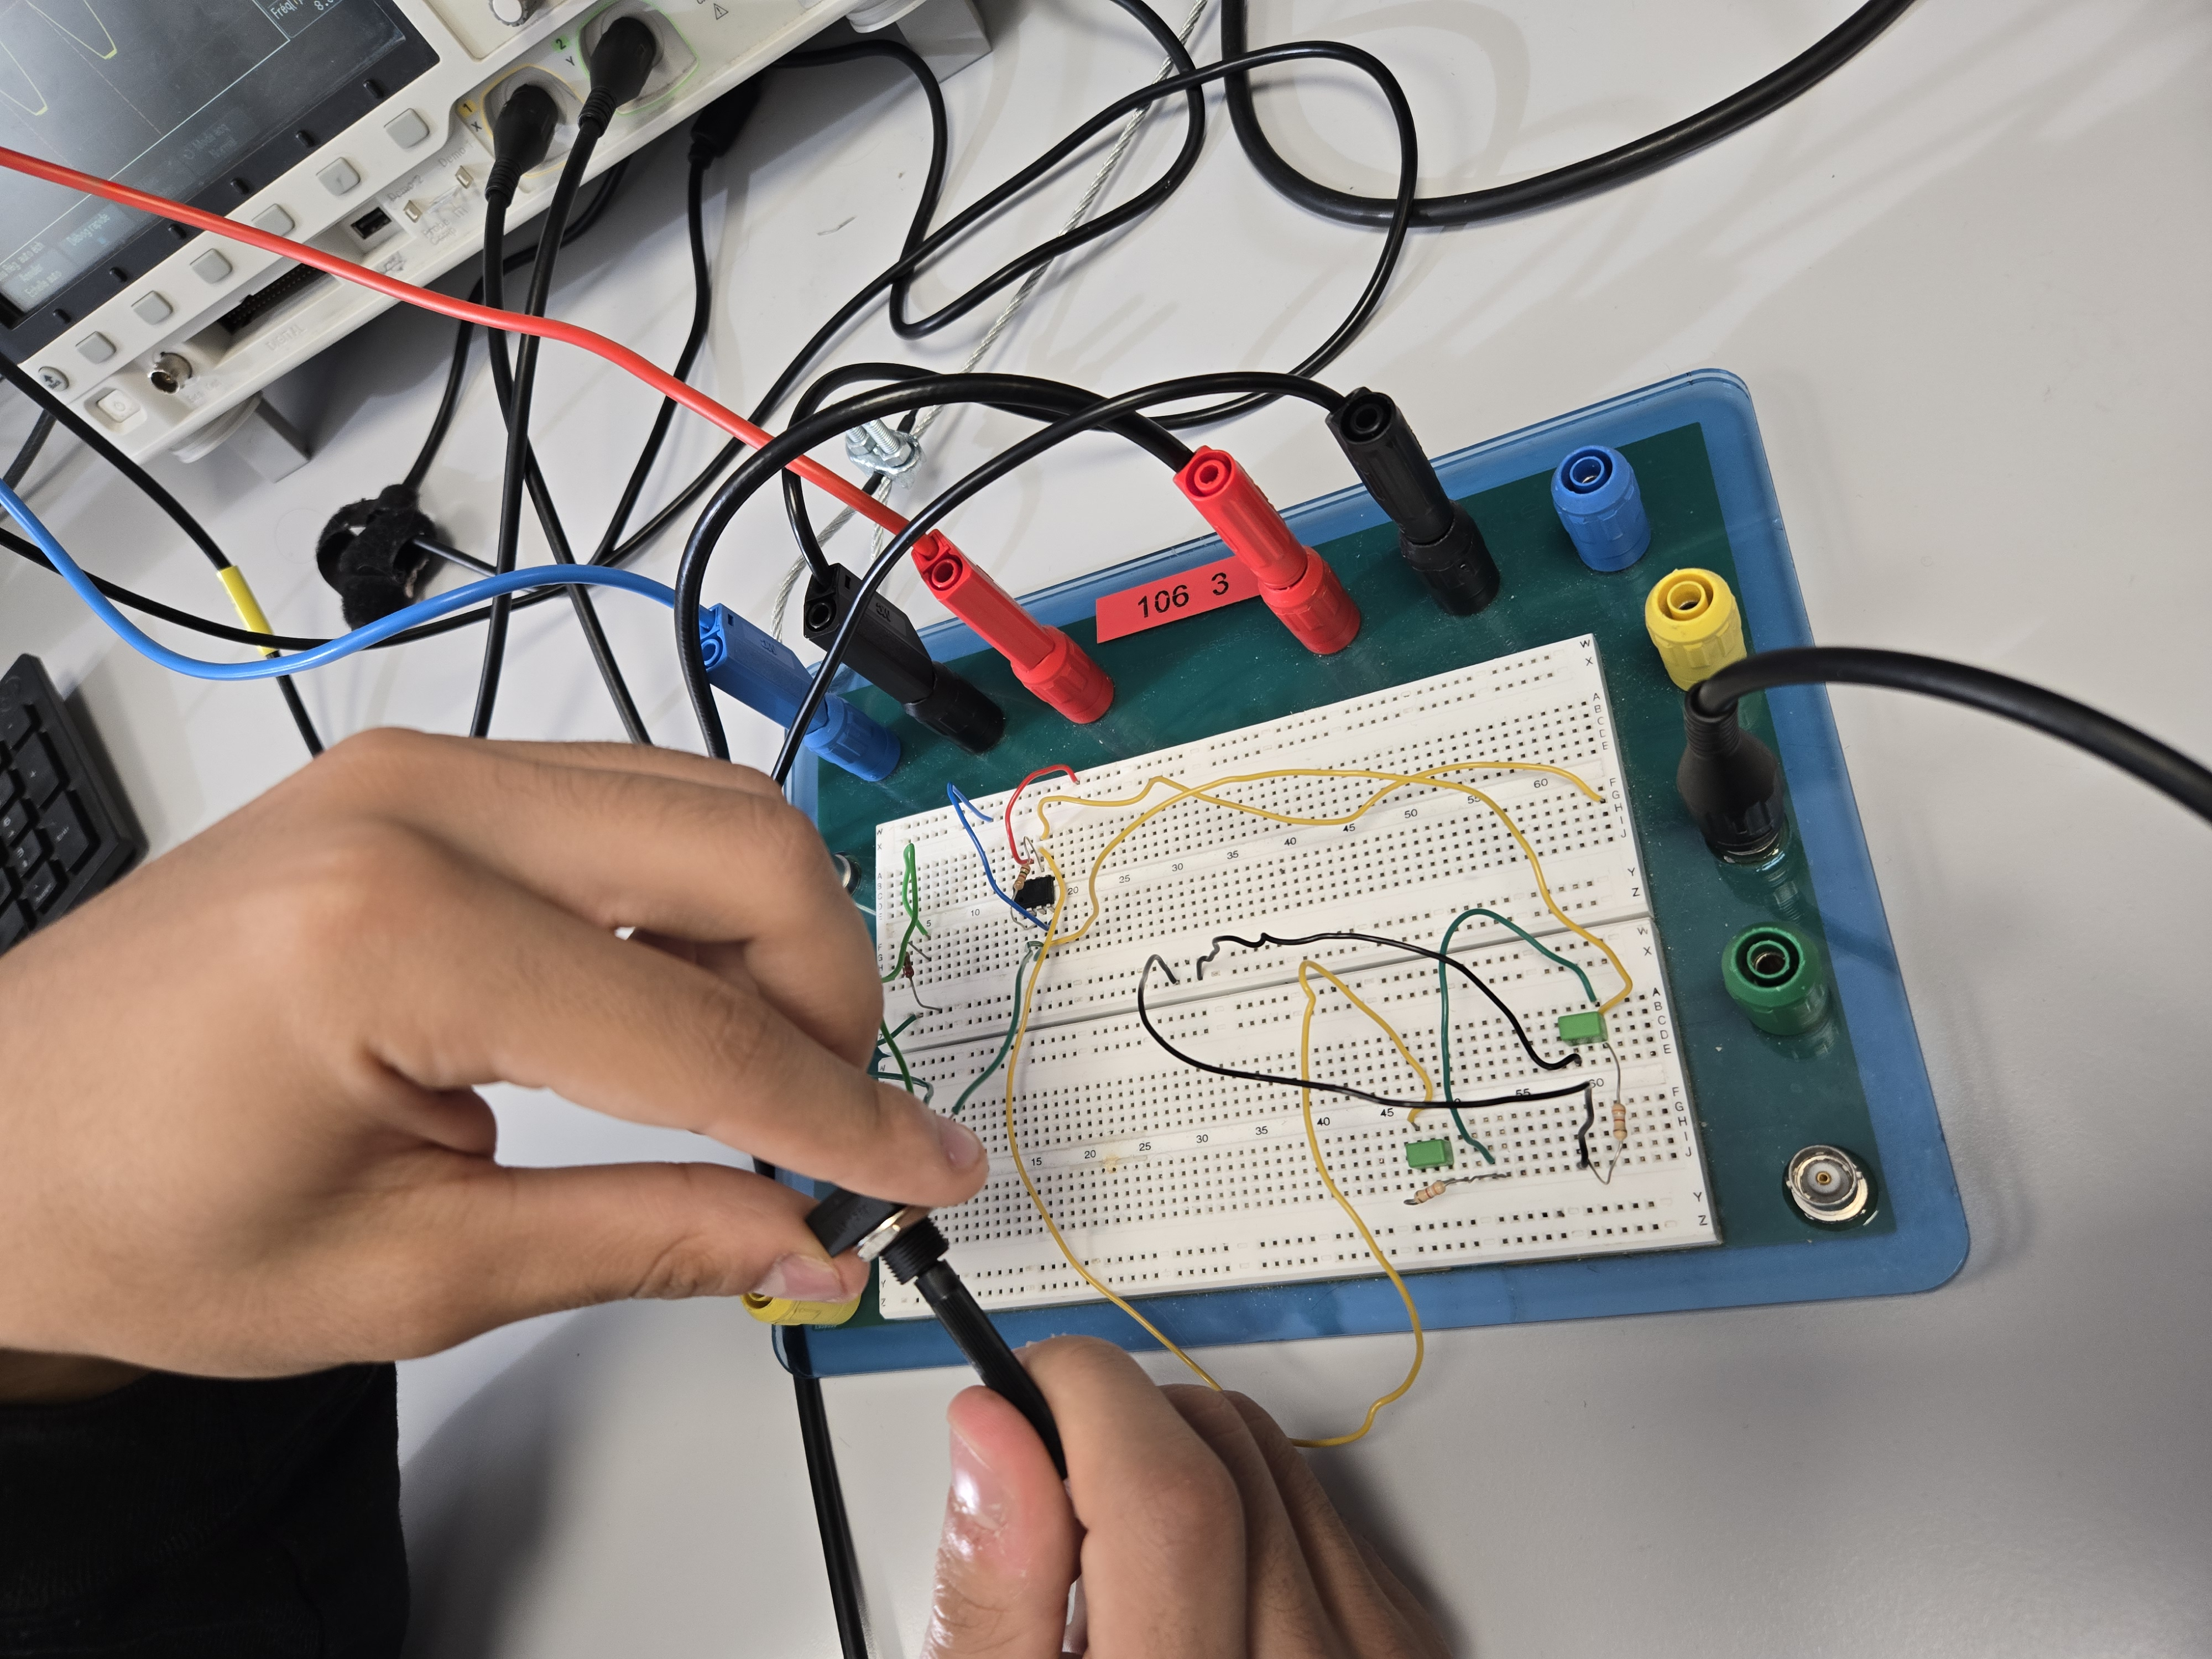
\includegraphics[width=0.78\linewidth]{images/montage_complet.jpg}
    \caption{Montage complet réalisé.}
\end{figure}

Le montage complet utilise un amplificateur non-inverseur. Pour satisfaire Barkhausen :
\[
A \cdot |\beta| = 1 \quad \Rightarrow \quad A = \frac{1}{|\beta|} \approx 3
\]
Nous avons câblé l'ampli avec $R_1 = \SI{220}{\ohm}$ en série avec un potentiomètre \SI{1}{\kilo\ohm} (réglable), et $R_2 = \SI{1.5}{\kilo\ohm}$ en tant que résistance fixe dans la configuration sujet.

\paragraph{Réglage}
En ajustant la résistance variable pour obtenir une oscillation sinusoïdale stable, on a trouvé un réglage pour lequel l'amplitude et la forme étaient satisfaisantes.

\paragraph{Mesures (oscillateur complet)}
\begin{table}[H]
\centering
\begin{tabular}{lcc}
\toprule
Grandeur & Mesure & Commentaire \\
\midrule
Fréquence d'oscillation (TL081) & \SI{8.86}{\kilo\hertz} & très proche de $f_{th}$ \\
Tension crête ($V_{p}$) & \SI{9.6}{\volt} & soit $V_{pp}\approx\SI{19.5}{\volt}$ \\
Forme d'onde & sinusoïde quasi-pure & vue sur l'oscillo \\
Comportement si $R_{var}$ augmenté & oscillations décroissent & $|A\beta|<1$ \\
Comportement si $R_{var}$ diminué & saturation / écrêtage & $|A\beta|>1$ \\
\bottomrule
\end{tabular}
\caption{Mesures et observations pour l'oscillateur à pont de Wien}
\end{table}

\begin{figure}[H]
    \centering
    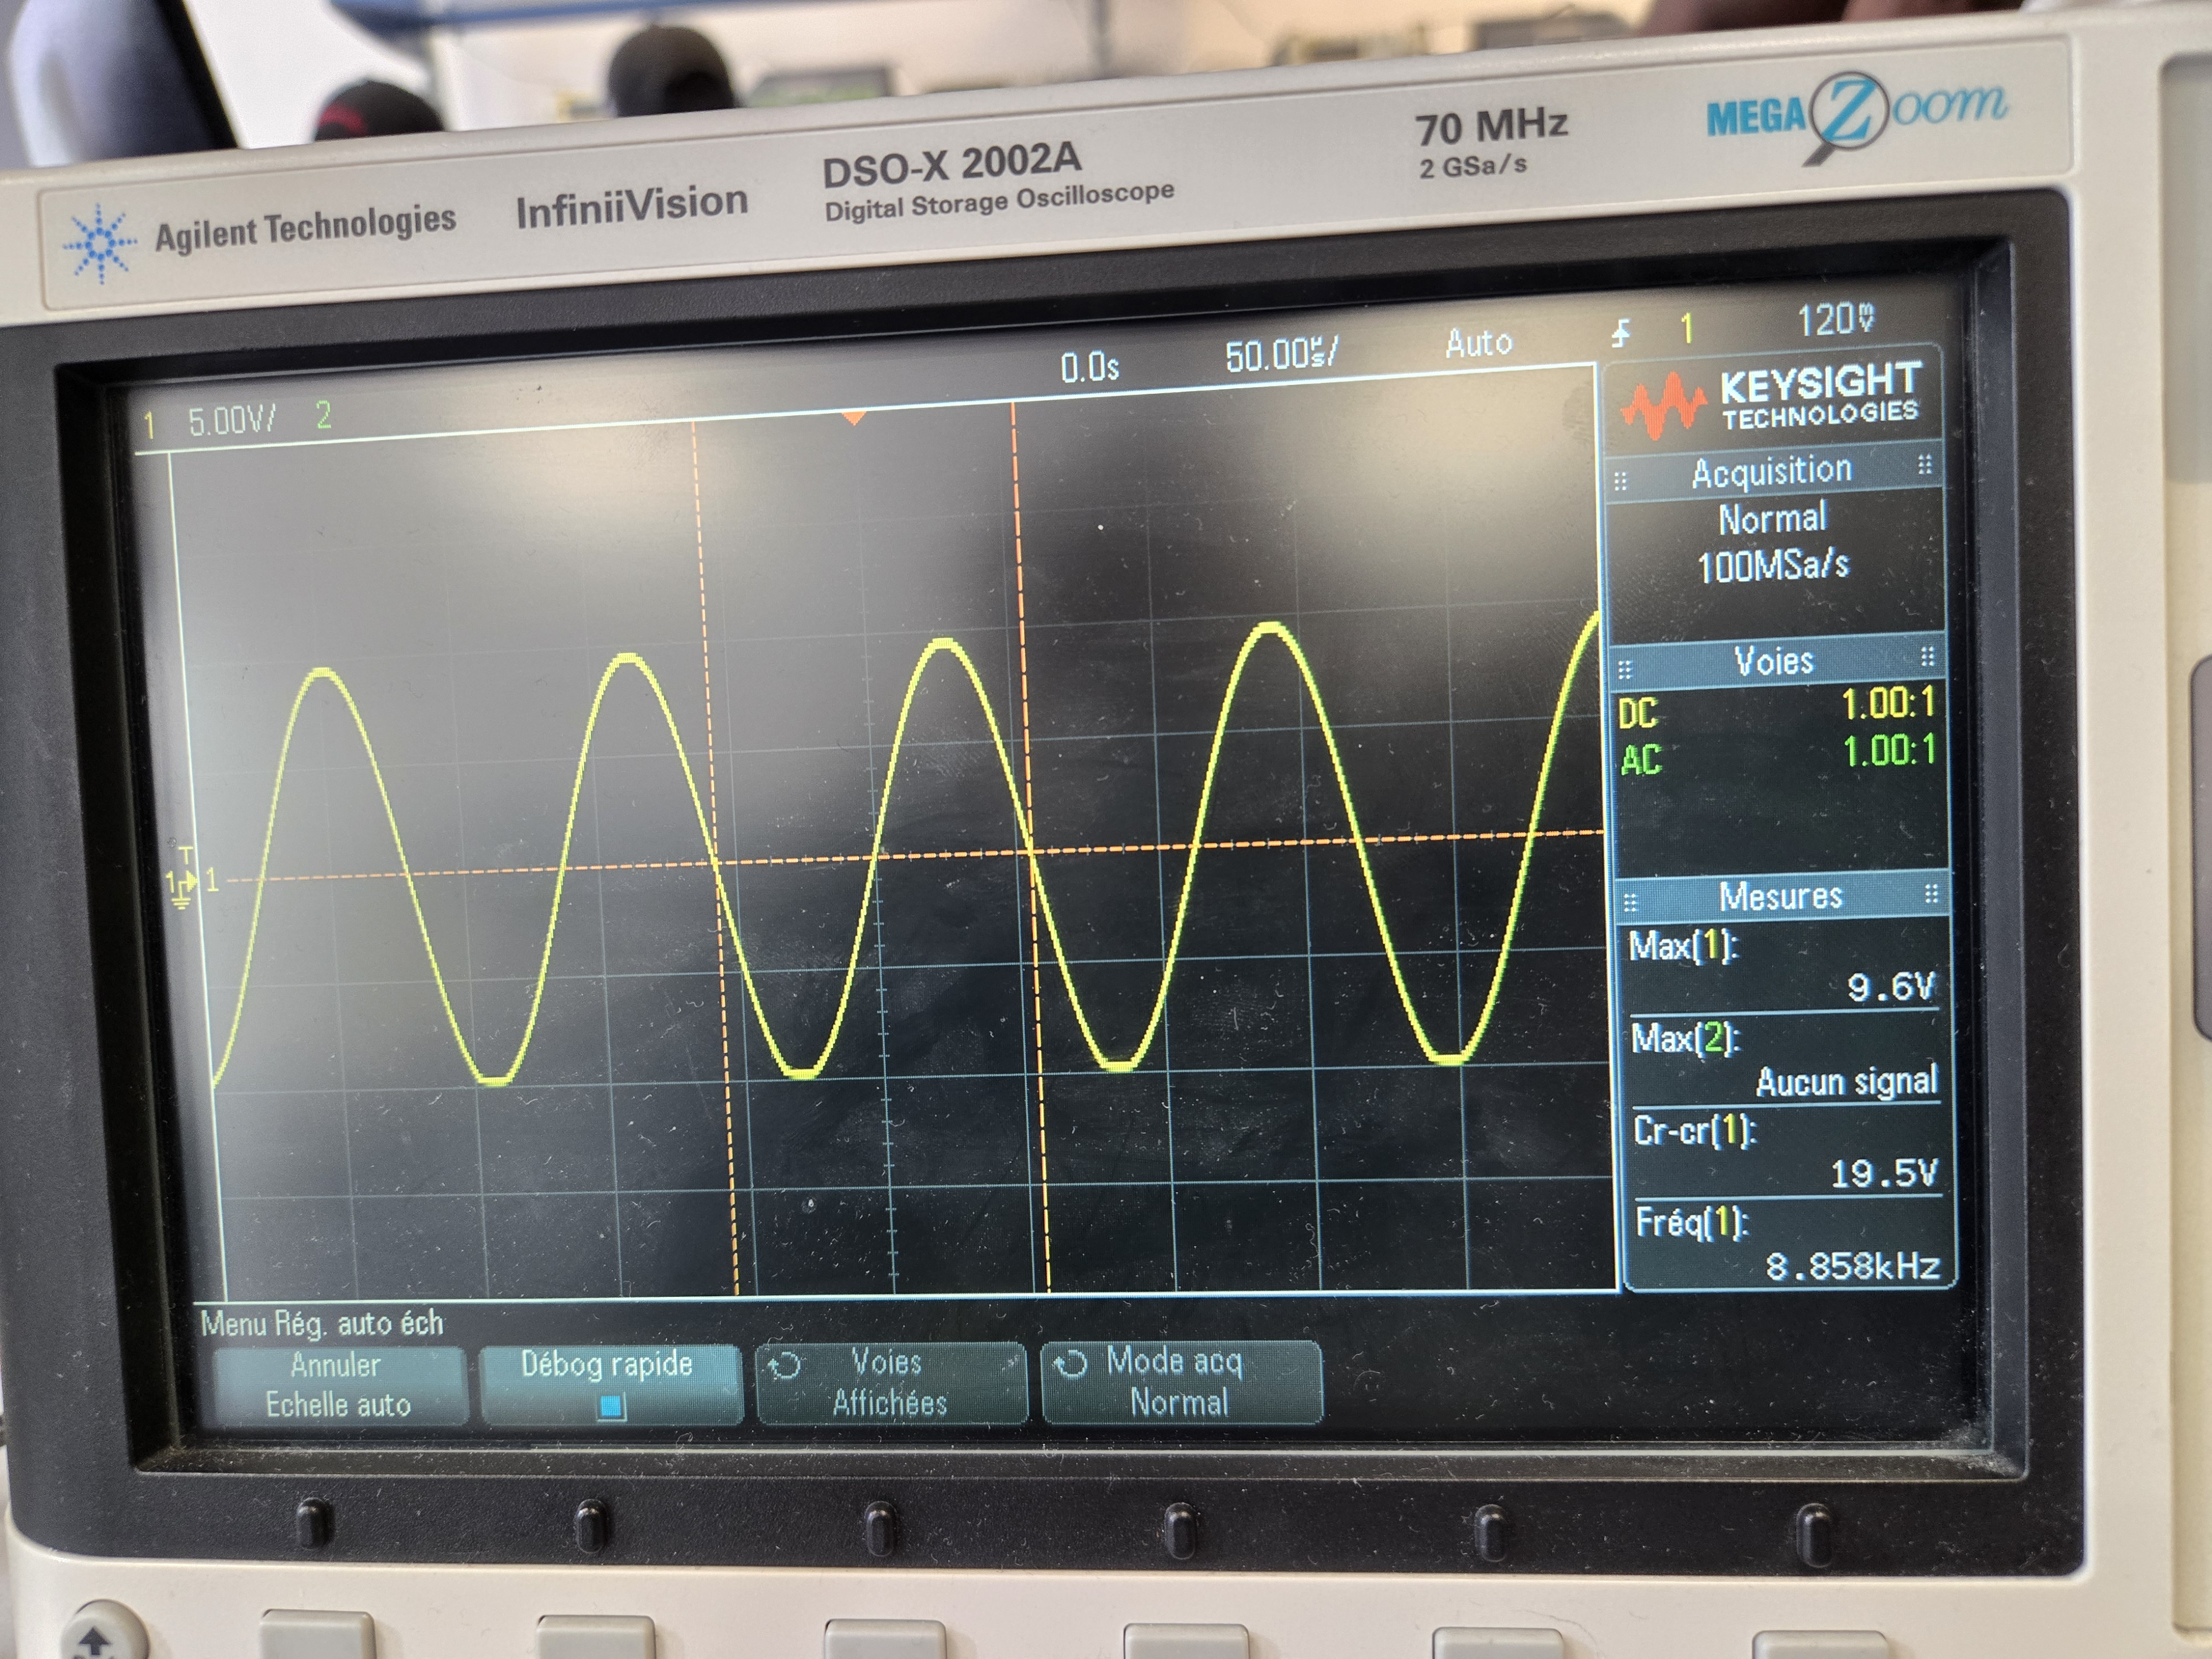
\includegraphics[width=0.78\linewidth]{images/oscillo_wien_temporal.jpg}
    \caption{Forme d'onde temporelle de sortie (TL081) — oscillations quasi-sinusoïdales.}
\end{figure}

\subsection{III -- Démarrage des oscillations (mode monocoup)}
Procédure :
\begin{enumerate}
    \item Régler le trigger proche de 0 V et sélectionner le mode ``single'' de l'oscilloscope.
    \item Couper l'alimentation, armer le déclenchement puis rallumer l'alimentation.
    \item Observer l'enregistrement : on visualise la montée en amplitude des premières périodes.
\end{enumerate}

\paragraph{Observation}
La séquence d'amorçage montre une croissance exponentielle initiale (bruit amplifié) jusqu'à la saturation de la boucle non-linéaire (stabilisation automatique si FET présent). Voir la figure ci-dessous.

\begin{figure}[H]
    \centering
    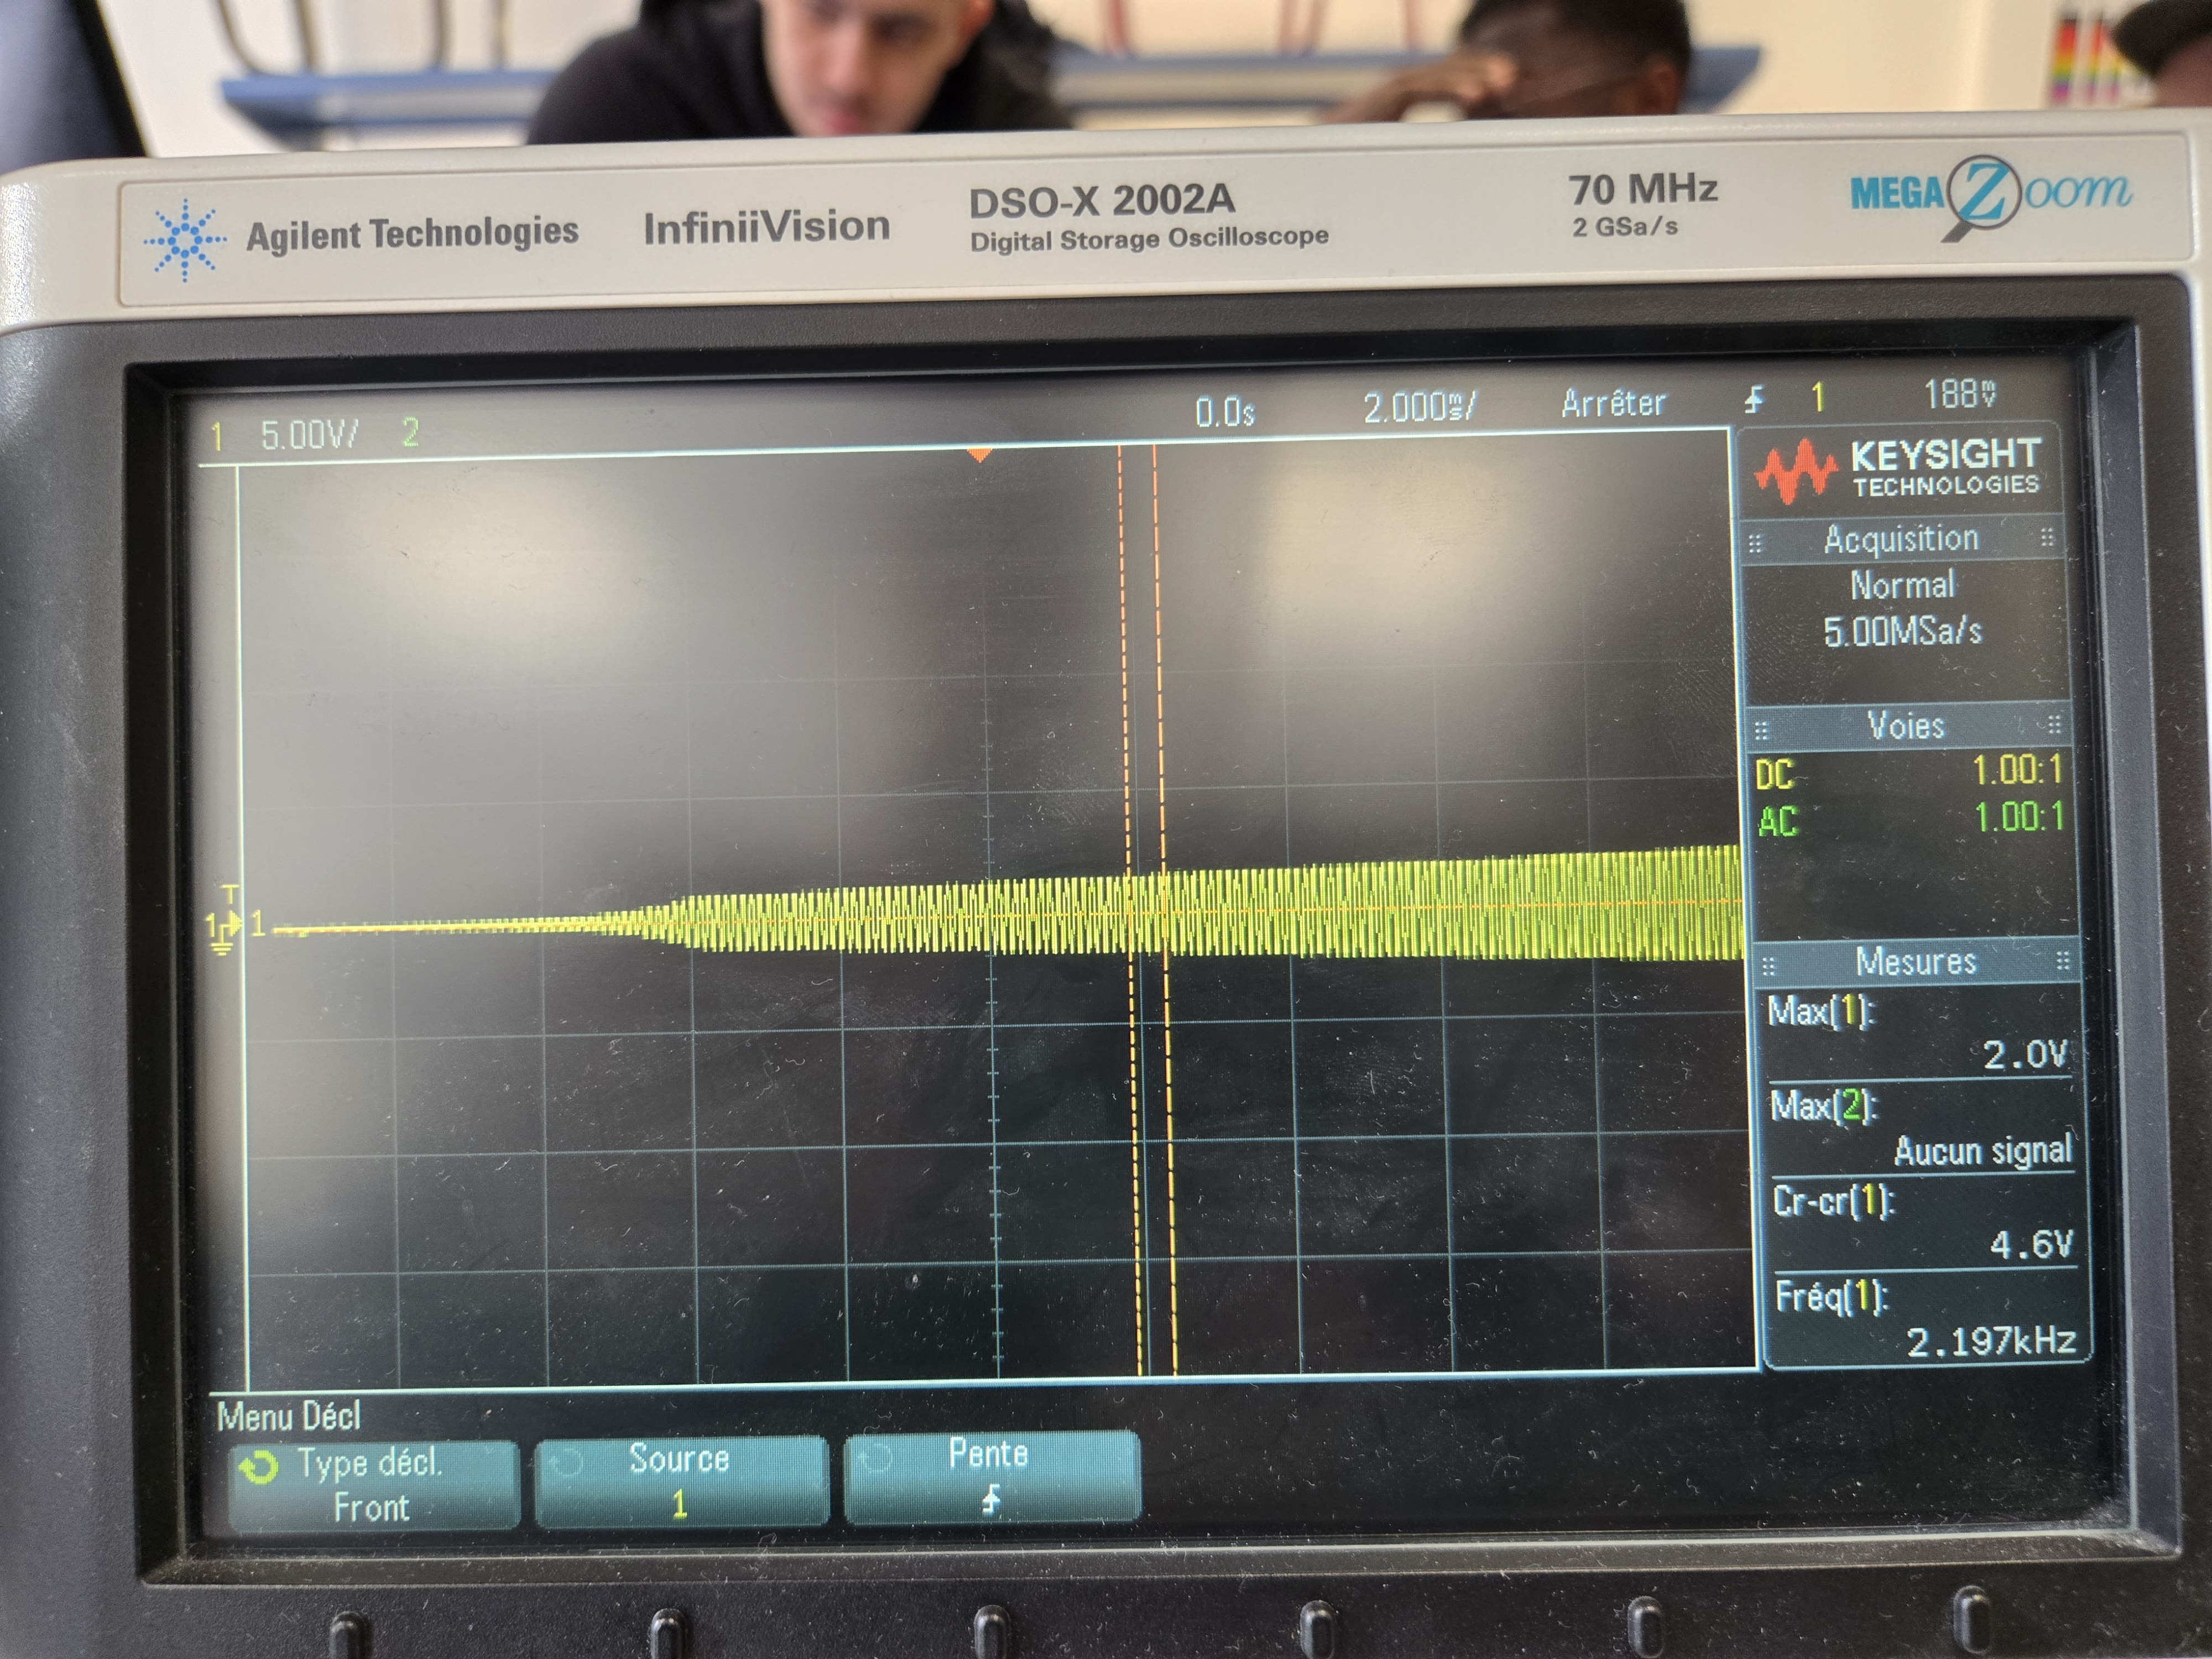
\includegraphics[width=0.78\linewidth]{images/oscillo_wien_demarrage.jpg}
    \caption{Démarrage des oscillations (mode monocoup) — montée en amplitude.}
\end{figure}

\subsection{IV -- Stabilisation de l'amplitude par résistance commandée (FET)}

\paragraph{Résistance commandée en tension}

Pour réaliser une résistance commandée en tension, nous avons mis en série une résistance fixe de \SI{470}{\ohm} et un JFET BF245C. Le JFET se comporte comme une résistance variable $R_{ds}$ dont la valeur dépend de la tension de grille $V_{gs}$. Plus $V_{gs}$ est négative, plus $R_{ds}$ augmente, et inversement.

La résistance totale du montage vaut alors :
\[
    R_{c} = 470 + R_{ds}
\]


\begin{figure}[H]
    \centering
    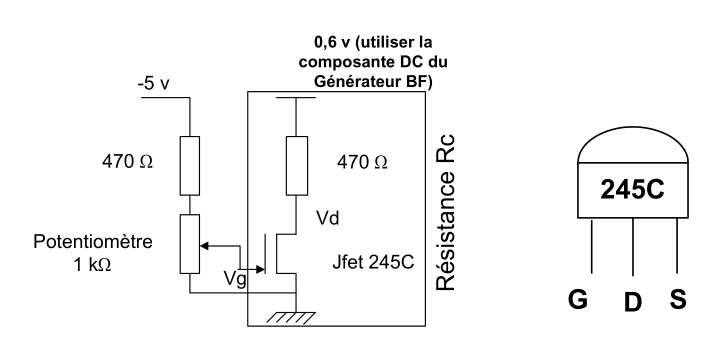
\includegraphics[width=0.9\linewidth]{images/schema_rc_vgs.png}
    \caption{Montage.}
\end{figure}

\paragraph{Caractérisation du FET}
Mesures réalisées sur banc : on mesure $R_{DS}$ (approximation) en fonction de $V_{GS}$ (tension de grille relative à la source) :

\begin{table}[H]
\centering
\begin{tabular}{|c|c|c|c|c|c|c|c|}
\hline
\textbf{R ($\Omega$)} & \textbf{Vds (V)} & \textbf{Vd (V)} & \textbf{Vg (V)} & \textbf{Id (mA)} & \textbf{R ($\Omega$)} & \textbf{Rds ($\Omega$)} & \textbf{Rc ($\Omega$)} \\

\hline
0 & 0 & 0.6 & 0 & 1.277 & 470 & 0 & 470 \\
\hline
518.367 & 0.199 & 0.6 & -0.52 & 0.853 & 470 & 233 & 703 \\
\hline
1017 & 0.214 & 0.6 & -1.02 & 0.821 & 470 & 261 & 731 \\
\hline
1496 & 0.231 & 0.6 & -1.5 & 0.785 & 470 & 294 & 764 \\
\hline
2030 & 0.253 & 0.6 & -2.01 & 0.738 & 470 & 343 & 813 \\
\hline
2502 & 0.281 & 0.6 & -2.52 & 0.679 & 470 & 414 & 884 \\
\hline
3019 & 0.317 & 0.6 & -2.99 & 0.602 & 470 & 527 & 997 \\
\hline
3505 & 0.351 & 0.6 & -3.4 & 0.530 & 470 & 662 & 1132 \\
\hline
\end{tabular}
\caption{Caractéristiques de la résistance commandée en tension}
\label{tab:rds_measurements}
\end{table}

\begin{figure}[H]
    \centering
    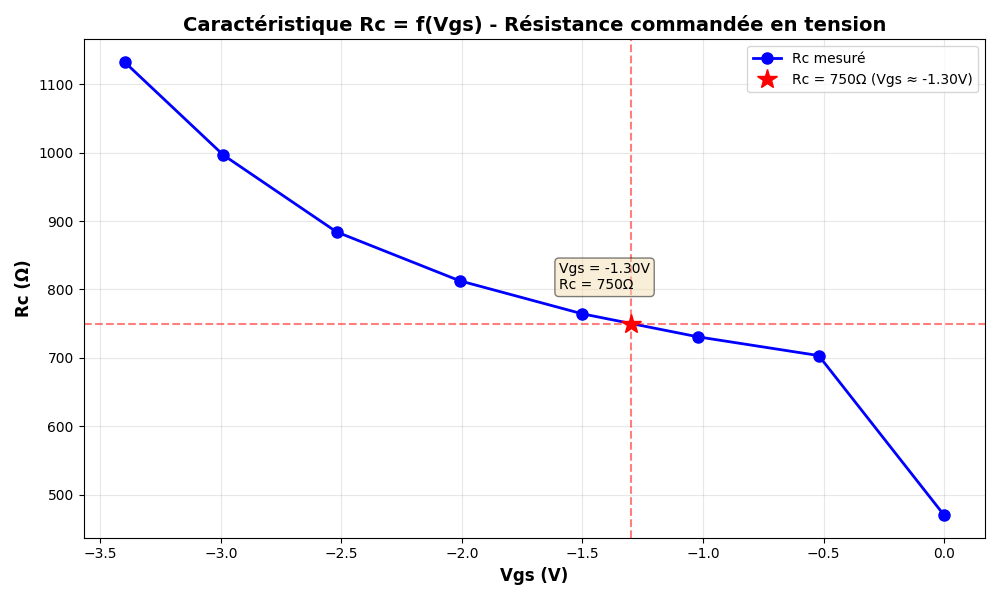
\includegraphics[width=0.9\linewidth]{images/rc_vgs.png}
    \caption{Courbe de Rc = f(Vgs).}
\end{figure}

D'après ces valeurs, la valeur approximative de $V_{GS}$ pour laquelle $R_{C}\approx \SI{750}{\ohm}$ est approximativement \(\mathbf{-1.3\ \text{V}}\).

\paragraph{Montage de génération de $V_g$}
Le détecteur est réalisé avec une diode (D1) suivi d'un filtre RC (r=10k + P1 k\(\Omega\), c=\SI{330}{\nano\farad}) et un potentiomètre P1 (\SI{10}{\kilo\ohm}) divisant la tension de détection pour obtenir la tension de grille $V_g$ (polarisée négativement si nécessaire selon le type de FET). Voir schéma.

\begin{figure}[H]
    \centering
    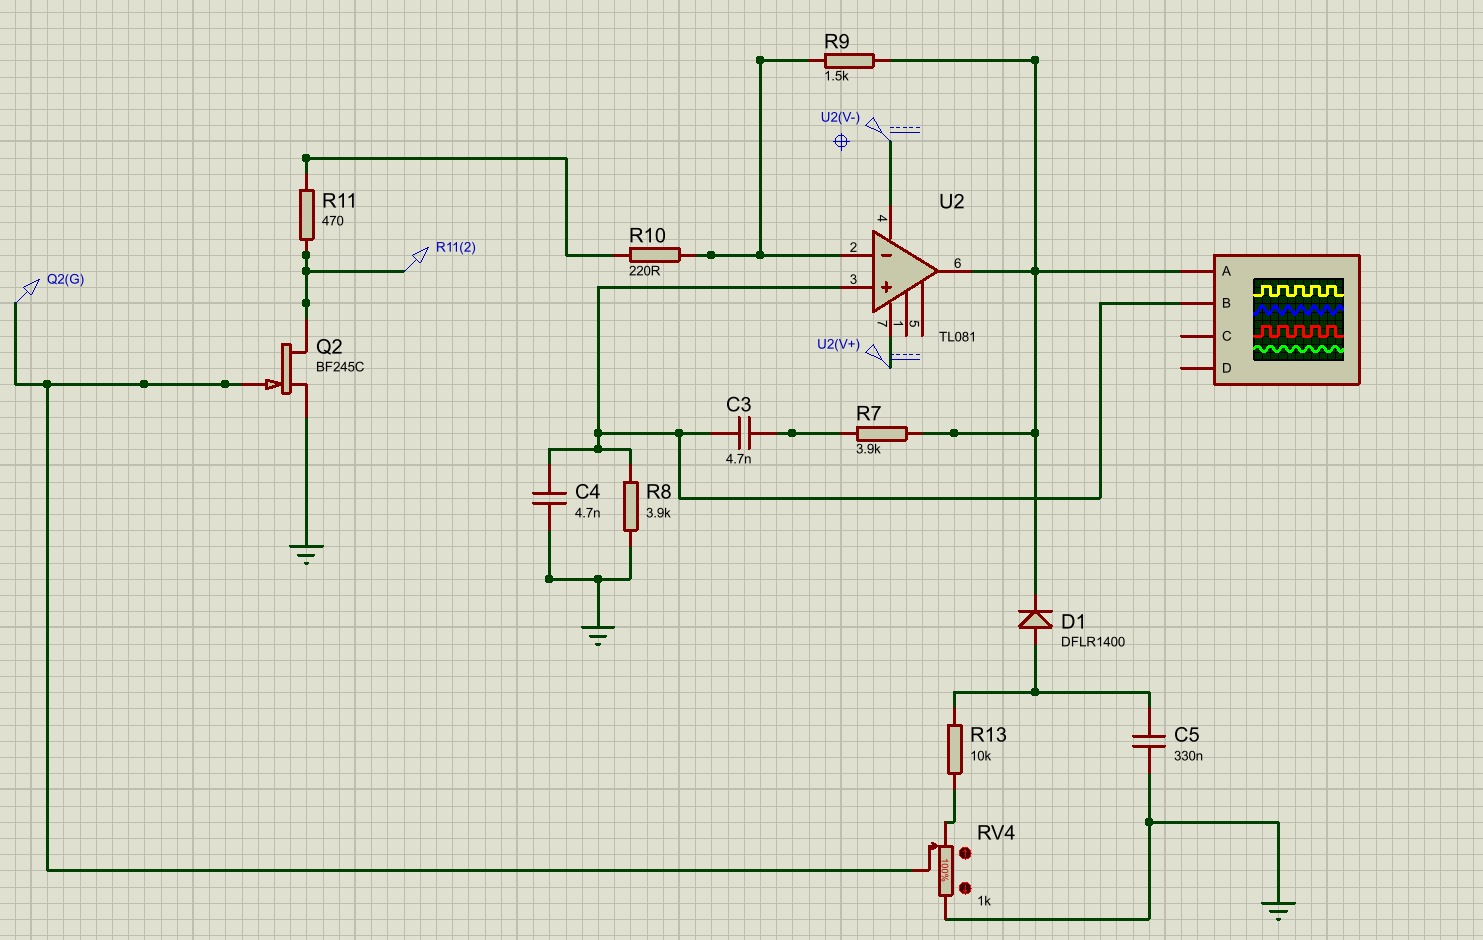
\includegraphics[width=0.9\linewidth]{images/dynamic_stabilisation.jpeg}
    \caption{Schéma du réseau de réaction avec stabilisation d'amplitude par JFET.}
    \label{fig:Schéma du réseau de réaction avec stabilisation d'amplitude par JFET}
\end{figure}



% \begin{figure}[H]
%     \centering
%     \includegraphics[width=0.78\linewidth]{images/oscillo_wien_fg.png}
%     \caption{Schéma du circuit de détection et commande $V_g$.}
%     \label{fig:wien_fet}
% \end{figure}

\paragraph{Intégration et réglages}
Après intégration, en ajustant P1 on obtient une stabilisation automatique de l'amplitude à \(V_{pp}\approx \SI{19.4}{\volt}\). Le système évite l'écrêtage excessif et maintient une forme sinusoïdale correcte.

\paragraph{Observation finale}
La boucle de régulation présente une légère dynamique (constante de temps \(\tau \approx \SI{10}{\milli\second}\)), suffisante pour filtrer la composante alternative et réagir sur l'amplitude moyenne sans produire d'oscillation de basse fréquence parasite.

\clearpage

% ---------- Partie III : Influence AOP ----------
\chapter{Influence des performances de l'amplificateur opérationnel}

\section{Caractéristiques des AOP testés}
\begin{table}[H]
\centering
\begin{tabular}{lcc}
\toprule
Amplificateur & GBW & Slew Rate (SR) \\
\midrule
TL081 & \SI{3}{\mega\hertz} & \SI{13}{\volt\per\micro\second} \\
$\mu$A741 & \SI{1}{\mega\hertz} & \SI{0.5}{\volt\per\micro\second} \\
\bottomrule
\end{tabular}
\caption{Caractéristiques fabricants (typique)}
\end{table}

\section{I -- Remplacement TL081 $\rightarrow$ $\mu$A741 (C = 4.7 nF)}
\paragraph{Mesure des fréquences}
\begin{itemize}
    \item \(f_{TL081} = \SI{8.65}{\kilo\hertz}\) (oscillateur stable, sinusoïde propre)
    \item \(f_{\mu A741} = \SI{8.52}{\kilo\hertz}\) (légère baisse due à la réponse en fréquence de l'ampli)
\end{itemize}

\paragraph{Analyse}
Le rapport relatif :
\[
\frac{f_{TL081} - f_{\mu A741}}{f_{th}} \approx \frac{8.65 - 8.52}{8.69} \approx 0.015 \quad (1.5\%)
\]
Ce rapport traduit la petite déformation de la réponse en boucle due au GBW limité du $\mu$A741. À \(\SI{8.7}{\kilo\hertz}\) les deux AOP fournissent encore un gain suffisant, mais la phase et le gain effectifs légèrement différents entraînent une petite variation de $f$.

\paragraph{Forme d'onde}
\begin{itemize}
    \item TL081 : sinusoïde quasi-idéale.
    \item $\mu$A741 : légère déformation des pentes (début d'écrêtage dans les régions de pente maximale) due au Slew Rate limité.
\end{itemize}

\section{II -- Remplacement des capacités (C = 1 nF)}
On remplace les condensateurs de \SI{4.7}{\nano\farad} par \SI{1}{\nano\farad}, ce qui augmente la fréquence d'oscillation d'environ un facteur \(4.7\).

\paragraph{Mesures}
\begin{itemize}
    \item \(f_{TL081}^{(C=1\text{nF})} \approx \SI{19.1}{\kilo\hertz}\)
    \item \(f_{\mu A741}^{(C=1\text{nF})} \approx \SI{18.2}{\kilo\hertz}\)
\end{itemize}

\paragraph{Slew Rate requis}
Pour \(V_{p}=\SI{3.6}{\volt}\) et \(f=\SI{19.1}{\kilo\hertz}\) :
\[
SR_{nécessaire} = V_p \cdot 2\pi f \approx 3.6 \times 2\pi \times 19100 \approx \SI{0.43}{\volt\per\micro\second}
\]
(ici on utilise \(V_p\) au lieu du pic maximal plus élevé pour une estimation)

\paragraph{Conclusion pratique}
\begin{itemize}
    \item TL081 (SR = \SI{13}{\volt\per\micro\second}) : largement suffisant, sinusoïde propre.
    \item $\mu$A741 (SR = \SI{0.5}{\volt\per\micro\second}) : SR proche du SR nécessaire → distorsion importante (triangle marqué), surtout à amplitude élevée.
\end{itemize}

\clearpage

% ---------- Partie B : Déphasage ----------
\chapter{Oscillateur à déphasage RC}

\section{Réseau RC et caractérisation}

\begin{figure}[H]
    \centering
    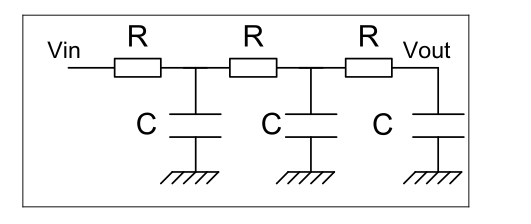
\includegraphics[width=0.78\linewidth]{images/reseau_rc.png}
    \caption{Schéma du montage réalisé sur notre plaque d'essai.}
\end{figure}

Réseau en cascade de 3 cellules RC identiques :
\[
R = \SI{1.8}{\kilo\ohm}, \qquad C = \SI{10}{\nano\farad}.
\]
La fréquence d'oscillation théorique (pour amplificateur inverseur) s'exprime :
\[
\omega_{osc} = \frac{\sqrt{6}}{RC}, \qquad f_{osc} = \frac{\sqrt{6}}{2\pi RC}.
\]
Calcul numérique :
\[
RC = 1.8\times 10^{3} \times 10\times 10^{-9} = 1.8\times 10^{-5},
\]
\[
f_{th} \approx \frac{2.4495}{2\pi \times 1.8\times 10^{-5}} \approx \SI{21.65}{\kilo\hertz}.
\]

\subsection{I -- Mesures sur le réseau (mode XY)}
En mode XY (entrée sur X, sortie sur Y), on recherche la fréquence où la phase nette vaut $-180^\circ$ (trace en opposition de phase).

\begin{table}[H]
\centering
\begin{tabular}{lcc}
\toprule
Grandeur & Mesure & Commentaire \\
\midrule
Fréquence théorique $f_{th}$ & \SI{21.65}{\kilo\hertz} & calculée \\
Fréquence mesurée $f_m$ (sans charge) & \SI{21.3}{\kilo\hertz} & alignement XY \\
Gain $|\beta|$ à $f_m$ & 0.034 & proche de $1/29$ théorique \\
\bottomrule
\end{tabular}
\caption{Mesures sur le réseau déphasant (sans charge)}
\end{table}

\begin{figure}[H]
    \centering
    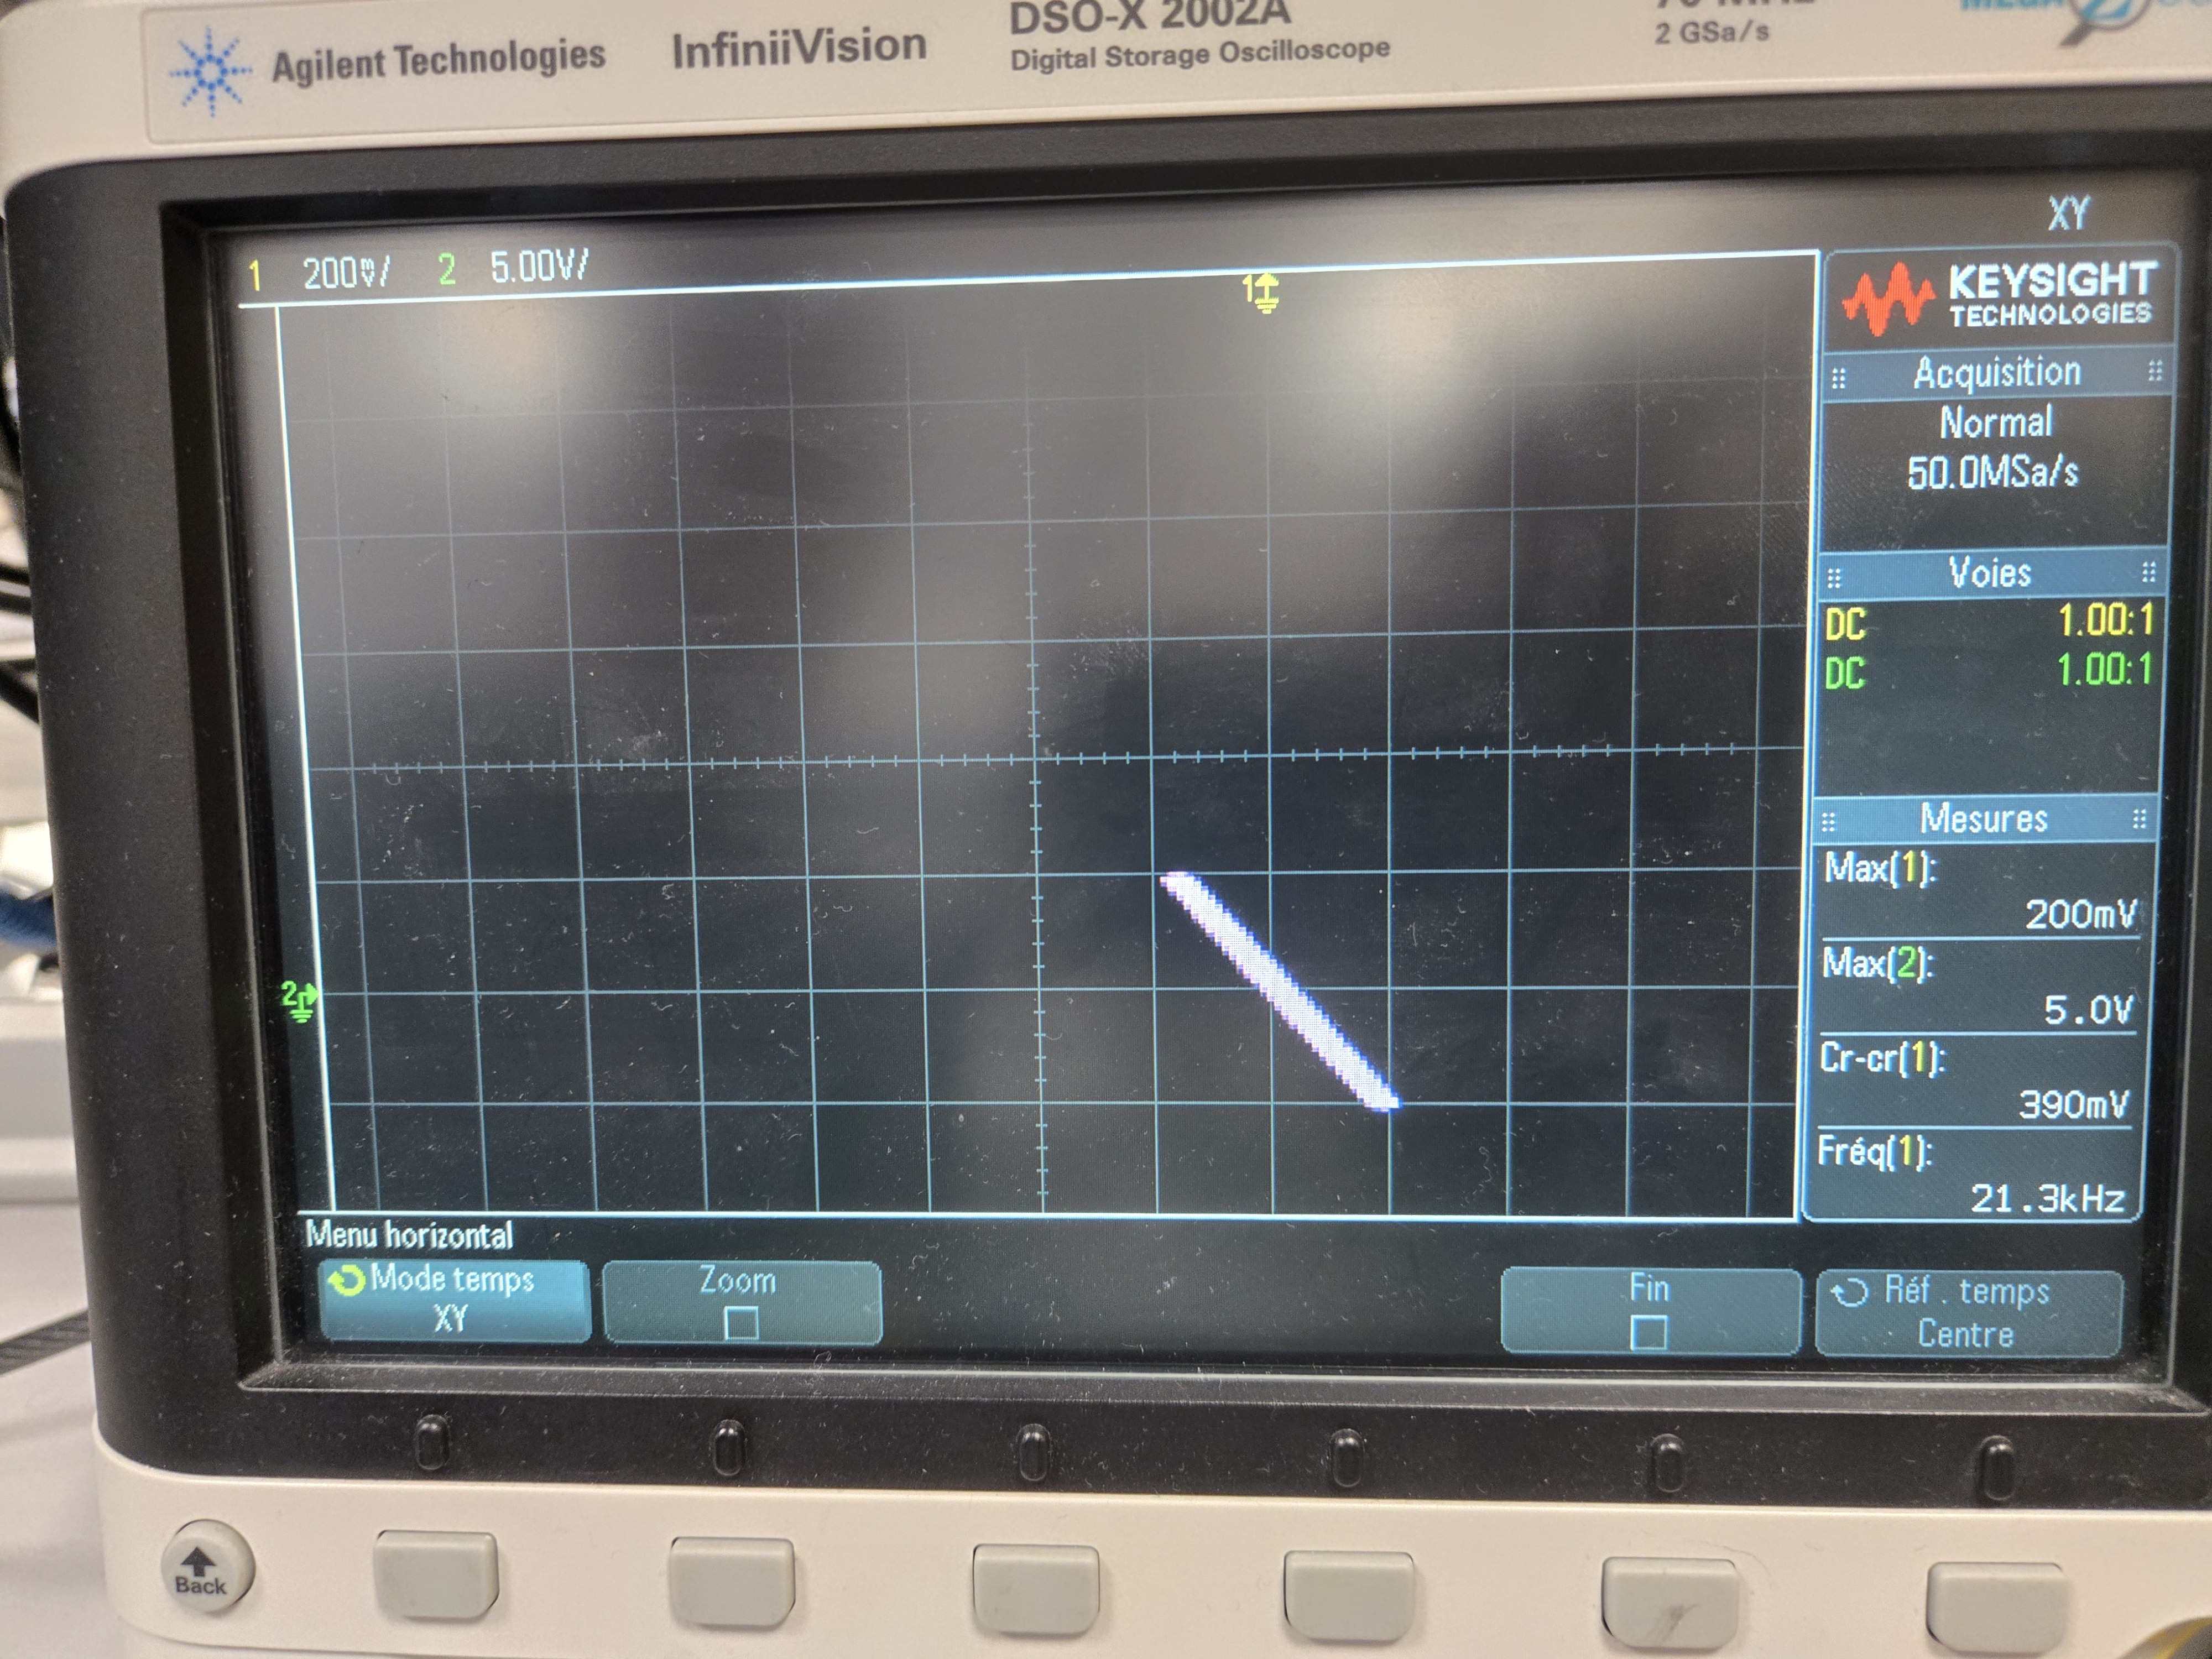
\includegraphics[width=0.78\linewidth]{images/oscillo_dephasage_xy.jpg}
    \caption{Tracé XY du réseau déphasant à $f\approx \SI{21.3}{\kilo\hertz}$.}
\end{figure}


\paragraph{Effet de la charge}
En chargeant la sortie par une résistance \(R_L=\SI{10}{\kilo\ohm}\), la fréquence diminue légèrement (par amortissement) : \(f \approx \SI{21.1}{\kilo\hertz}\). Avec \(R_L=\SI{1}{\kilo\ohm}\) la chute est plus importante et l'atténuation augmente (risque de ne plus pouvoir compenser avec un gain raisonnable).

\subsection{II -- Montage complet (amplificateur inverseur)}
\begin{figure}[H]
    \centering
    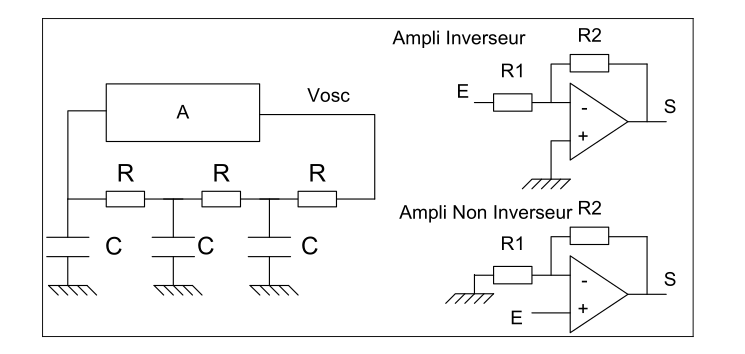
\includegraphics[width=0.78\linewidth]{images/reseau_rc_complet.png}
    \caption{Schéma du réseau RC Complet.}
\end{figure}
Pour l'oscillateur on utilise un amplificateur inverseur. La valeur de gain nécessaire (théorique) :
\[
|\beta| = \frac{1}{29} \quad \Rightarrow \quad A = 29.
\]
Avec \(R_1=\SI{10}{\kilo\ohm}\) (entrée) on a \(R_2\approx 290\ \text{k}\Omega\) (amplificateur inverseur : \(A=-R_2/R_1\)).

\paragraph{Mesures (oscillateur complet)}
\begin{itemize}
    \item Réglage trouvé pour oscillation : \(R_2 = \SI{290}{\kilo\ohm}\) (résistance fixe + pot).
    \item Fréquence mesurée d'oscillation : \(f_{osc} \approx \SI{21.4}{\kilo\hertz}\) (très proche de $f_{th}$).
    \item Tension de sortie \(V_{pp}\) : \(\approx\SI{6.8}{\volt}\) (sinusoïde acceptable).
\end{itemize}



\subsection{III -- Variations de R1 et conclusions pratiques}
On a répété l'expérience en prenant \(R_1=\SI{1}{\kilo\ohm}\) (et \(R_2\) ajusté avec pot 10 k\(\Omega\)). :
\begin{itemize}
    \item L'oscillation est obtenue, mais le réglage de \(R_2\) devient plus sensible ; la stabilité en amplitude est moins bonne (sensibilité aux perturbations).
    \item La fréquence reste essentiellement identique (dépend du produit \(RC\)), ce qui confirme la théorie.
\end{itemize}

\clearpage

% ---------- Analyse générale ----------
\chapter{Analyse des résultats}

\section{Validation des fréquences d'oscillation}

\subsection{Oscillateur à pont de Wien}

Les mesures effectuées sur l'oscillateur à pont de Wien montrent une très bonne concordance avec la théorie. Avec des composants \(R = \SI{3.9}{\kilo\ohm}\) et \(C = \SI{4.7}{\nano\farad}\), nous avons obtenu une fréquence théorique de \SI{8.69}{\kilo\hertz}. La fréquence mesurée expérimentalement est de \SI{8.90}{\kilo\hertz} pour le réseau seul, et \SI{8.86}{\kilo\hertz} pour l'oscillateur complet avec le TL081.

L'écart relatif entre la théorie et la mesure est d'environ :
\[
\epsilon = \frac{|f_{mes} - f_{th}|}{f_{th}} \approx \frac{|8.86 - 8.69|}{8.69} \approx 2\%
\]

Cet écart peut s'expliquer par plusieurs facteurs :
\begin{itemize}
    \item Les tolérances des composants passifs (résistances et condensateurs ont généralement une tolérance de 5 à 10\%)
    \item L'influence des capacités parasites du montage sur breadboard
    \item La légère charge introduite par l'impédance d'entrée de l'oscilloscope
\end{itemize}

Le rapport d'atténuation mesuré \(|\beta| = 0.333\) correspond exactement à la valeur théorique de \(1/3\) attendue pour un pont de Wien à la fréquence de résonance. Cela confirme que notre réseau fonctionne correctement et que la phase est bien nulle à cette fréquence.

\subsection{Oscillateur à déphasage}

Pour l'oscillateur à déphasage, avec \(R = \SI{1.8}{\kilo\ohm}\) et \(C = \SI{10}{\nano\farad}\), la fréquence théorique calculée est \SI{21.65}{\kilo\hertz}. Nous avons mesuré \SI{21.3}{\kilo\hertz} pour le réseau seul et \SI{21.4}{\kilo\hertz} pour l'oscillateur complet.

L'écart relatif est :
\[
\epsilon = \frac{|21.4 - 21.65|}{21.65} \approx 1.2\%
\]

Cette précision est encore meilleure que pour le pont de Wien, probablement parce que les valeurs des composants sont plus éloignées de leurs limites basses fréquences (moins d'effets parasites). L'atténuation mesurée \(|\beta| = 0.034\) est très proche de la valeur théorique \(1/29 \approx 0.0345\), ce qui valide notre analyse théorique du réseau RC en cascade.

\section{Vérification de la condition de Barkhausen}

\subsection{Condition d'amplitude}

Pour que les oscillations s'auto-entretiennent, il faut que \(|A\beta| = 1\). Dans le cas du pont de Wien, avec \(|\beta| = 1/3\), nous devons avoir un gain \(A = 3\). En pratique, nous avons constaté que :
\begin{itemize}
    \item Si le gain est légèrement inférieur à 3 (en augmentant la résistance variable), les oscillations s'amortissent progressivement jusqu'à disparaître
    \item Si le gain dépasse 3 (en diminuant la résistance), l'amplitude augmente jusqu'à saturation, provoquant un écrêtage du signal
\end{itemize}

Cette observation confirme parfaitement la théorie : le système n'oscille de manière stable que lorsque le produit \(|A\beta|\) est très proche de 1.

Pour l'oscillateur à déphasage, avec \(|\beta| = 1/29\), nous avons dû ajuster le gain à environ 29 en utilisant \(R_1 = \SI{10}{\kilo\ohm}\) et \(R_2 = \SI{290}{\kilo\ohm}\). Le réglage s'est avéré plus délicat car la plage de réglage pour obtenir une oscillation stable est plus étroite (sensibilité accrue).

\begin{figure}[H]
    \centering
    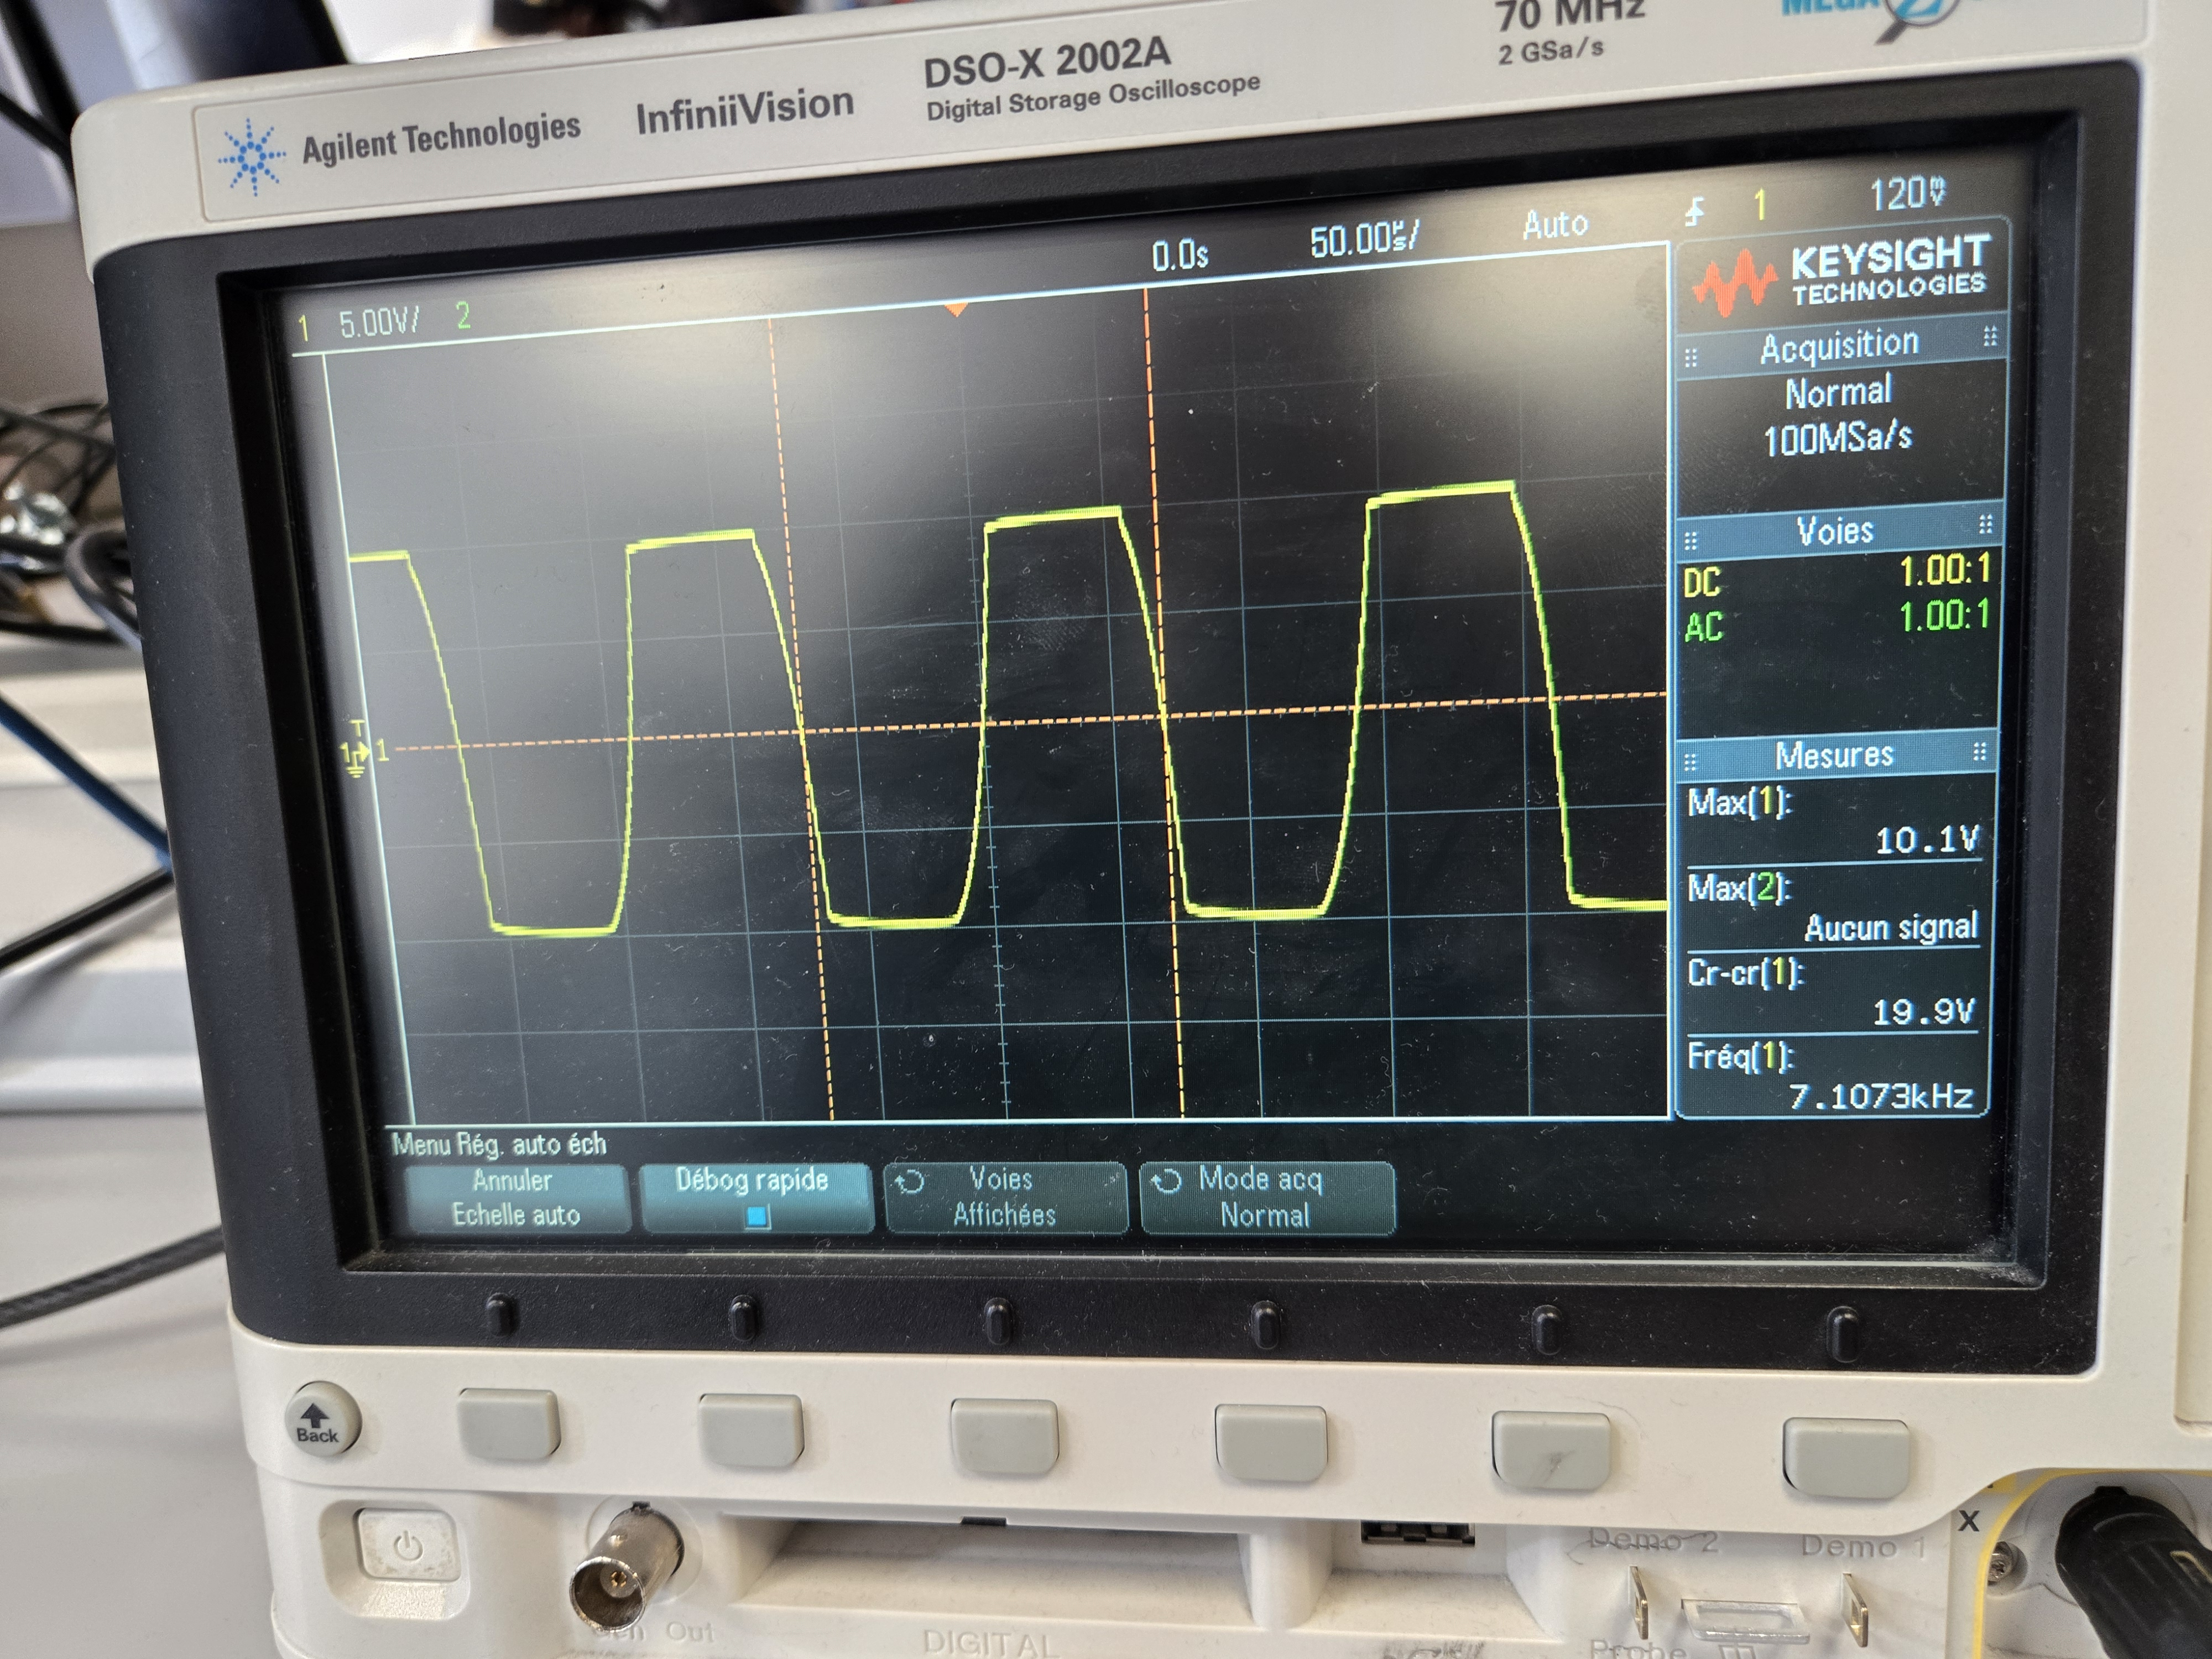
\includegraphics[width=0.78\linewidth]{images/ecretage.jpg}
    \caption{Ecretage.}
\end{figure}

\subsection{Condition de phase}

Les mesures en mode XY ont permis de vérifier la condition de phase. Pour le pont de Wien, la phase du réseau est nulle à la fréquence d'oscillation (trace alignée sur l'oscilloscope). Pour l'oscillateur à déphasage, le réseau introduit un déphasage de \(-180^\circ\), compensé par l'amplificateur inverseur qui ajoute \(-180^\circ\) supplémentaires, donnant ainsi un déphasage total de \(-360^\circ \equiv 0^\circ\) dans la boucle.

\section{Stabilisation d'amplitude par JFET}

\subsection{Caractérisation de la résistance commandée}

Les mesures effectuées sur le JFET BF245C montrent clairement la variation de \(R_{ds}\) en fonction de \(V_{gs}\). Nous avons observé que :
\begin{itemize}
    \item Pour \(V_{gs} = 0\text{V}\), le canal est complètement ouvert : \(R_{ds} \approx 0\ \Omega\)
    \item Pour \(V_{gs} = -3.4\text{V}\), le canal est presque fermé : \(R_{ds} \approx 662\ \Omega\)
\end{itemize}

La résistance effective totale \(R_{c} = 470 + R_{ds}\) varie donc entre \SI{470}{\ohm} et \SI{1132}{\ohm}. Cette plage de variation est suffisante pour permettre un contrôle efficace du gain de l'amplificateur.

D'après notre courbe \(R_{c} = f(V_{gs})\), nous avons déterminé qu'une tension de grille d'environ \SI{-1.3}{\volt} permet d'obtenir \(R_{c} \approx \SI{750}{\ohm}\), ce qui correspond au point de fonctionnement optimal pour notre oscillateur.

\subsection{Efficacité de la stabilisation}

L'intégration du système de stabilisation automatique (diode de détection + filtre RC + JFET) s'est révélée très efficace. Sans ce système, l'amplitude des oscillations variait fortement en fonction des conditions (température, dérive des composants). Avec la stabilisation, nous avons obtenu une amplitude constante de \(V_{pp} \approx \SI{19.4}{\volt}\) avec une forme sinusoïdale propre, sans écrêtage excessif.

La constante de temps du filtre RC (\(\tau \approx \SI{10}{\milli\second}\)) est bien choisie : elle est suffisamment grande pour ne pas suivre les variations instantanées du signal (qui oscillerait sinon à basse fréquence), mais assez petite pour réagir rapidement aux variations d'amplitude lentes.

\section{Influence des caractéristiques de l'amplificateur}

\subsection{Effet du produit gain-bande (GBW)}

Le remplacement du TL081 (GBW = \SI{3}{\mega\hertz}) par le \(\mu\)A741 (GBW = \SI{1}{\mega\hertz}) a entraîné une légère diminution de la fréquence d'oscillation : de \SI{8.65}{\kilo\hertz} à \SI{8.52}{\kilo\hertz}, soit une variation de 1.5\%.

Cette variation s'explique par le fait que, à la fréquence d'oscillation, le gain de l'amplificateur n'est plus infini. Le gain en boucle ouverte du \(\mu\)A741 à \SI{8.5}{\kilo\hertz} est d'environ :
\[
A_{BO} \approx \frac{GBW}{f} = \frac{10^6}{8.5 \times 10^3} \approx 118
\]

Ce gain reste largement supérieur au gain en boucle fermée nécessaire (environ 3), mais la limitation en fréquence introduit un léger déphasage supplémentaire qui décale légèrement la fréquence d'oscillation.

\subsection{Effet du Slew Rate}

L'effet du Slew Rate est particulièrement visible lorsque nous avons remplacé les condensateurs de \SI{4.7}{\nano\farad} par \SI{1}{\nano\farad}, augmentant ainsi la fréquence à environ \SI{19}{\kilo\hertz}.

Pour une sinusoïde de \(V_p = \SI{3.6}{\volt}\) à \SI{19.1}{\kilo\hertz}), la pente maximale est :
\[
\frac{dV}{dt}_{max} = V_p \cdot 2\pi f = 3.6 \times 2\pi \times 19100 \approx \SI{0.43}{\volt\per\micro\second}
\]

Le TL081, avec un SR de \SI{13}{\volt\per\micro\second}, peut suivre cette pente sans problème. Par contre, le \(\mu\)A741 (SR = \SI{0.5}{\volt\per\micro\second}) est à la limite de ses capacités. Nous avons effectivement observé une distorsion importante de la forme d'onde avec le \(\mu\)A741 : le signal tend vers une forme triangulaire car l'amplificateur ne peut pas suivre les variations rapides du signal sinusoïdal.

Cette limitation du Slew Rate est donc critique pour les applications haute fréquence ou grande amplitude. Dans notre cas, le TL081 est clairement plus adapté que le \(\mu\)A741 pour des fréquences supérieures à \SI{10}{\kilo\hertz}.

\section{Comportement dynamique et démarrage}

L'observation du démarrage des oscillations en mode monocoup a révélé un comportement intéressant. Au moment de la mise sous tension, le bruit électronique présent dans le circuit (tension thermique, bruit de quantification) est amplifié par la boucle. Si \(|A\beta| > 1\), cette composante à la fréquence de résonance croît exponentiellement jusqu'à ce qu'un mécanisme non-linéaire (saturation naturelle de l'ampli ou stabilisation par FET) limite l'amplitude.

Sans stabilisation, nous avons observé que l'amplitude met environ 50 à 100 périodes pour se stabiliser, avec un écrêtage final dû à la saturation. Avec le système de stabilisation par JFET, l'amplitude se stabilise plus rapidement (environ 20 périodes) à un niveau inférieur à la saturation, donnant une sinusoïde propre.

\section{Synthèse comparative}

\begin{table}[H]
\centering
\begin{tabular}{lcc}
\toprule
\textbf{Critère} & \textbf{Pont de Wien} & \textbf{Déphasage RC} \\
\midrule
Précision en fréquence & Excellente (2\%) & Excellente (1.2\%) \\
Facilité de réglage & Facile & Délicate \\
Stabilité d'amplitude & Bonne (avec FET) & Moyenne \\
Qualité du signal & Très bonne & Bonne \\
Sensibilité aux composants & Faible & Moyenne \\
Nombre de composants & Modéré & Élevé (3 cellules RC) \\
\bottomrule
\end{tabular}
\caption{Comparaison des deux architectures d'oscillateurs}
\end{table}

Dans l'ensemble, le pont de Wien s'avère plus facile à mettre en œuvre et plus stable, surtout avec le système de régulation d'amplitude. L'oscillateur à déphasage nécessite un gain plus élevé (29 au lieu de 3), ce qui le rend plus sensible aux variations de composants et plus difficile à stabiliser. Cependant, les deux architectures donnent des résultats satisfaisants et confirment parfaitement la théorie des oscillateurs linéaires.
\clearpage


\end{document}
